% vim: set spell spelllang=en tw=100 et sw=4 sts=4 foldmethod=marker foldmarker={{{,}}} :

\documentclass[aspectratio=169,compress,10pt]{beamer}

\usepackage{tikz}
\usepackage{xcolor}
\usepackage{complexity}
\usepackage{hyperref}
\usepackage{microtype}
\usepackage{amsmath}                   % \operatorname
\usepackage{amsfonts}                  % \mathcal
\usepackage{amssymb}                   % \nexists
\usepackage[vlined]{algorithm2e} % algorithms
\usepackage{centernot}
\usepackage{listings}
\usepackage{csquotes}
\usepackage{fancyvrb}
\usepackage{bussproofs}
\usepackage{multicol}
\usepackage{booktabs}
\usepackage{mathtools}
\usepackage{pifont}
\usepackage{marvosym}
\usepackage{cancel}
\usepackage{nicefrac}

\usefonttheme{professionalfonts}

\usetikzlibrary{shapes, arrows, shadows, calc, positioning, fit, decorations.pathreplacing,
decorations.pathmorphing, shapes.misc, tikzmark, backgrounds, trees, overlay-beamer-styles}

\definecolor{uofguniversityblue}{rgb}{0, 0.219608, 0.396078}
\definecolor{uofgheather}{rgb}{0.356863, 0.32549, 0.490196}
\definecolor{uofgaquamarine}{rgb}{0.603922, 0.72549, 0.678431}
\definecolor{uofgslate}{rgb}{0.309804, 0.34902, 0.380392}
\definecolor{uofgrose}{rgb}{0.823529, 0.470588, 0.709804}
\definecolor{uofgmocha}{rgb}{0.709804, 0.564706, 0.47451}
\definecolor{uofgsandstone}{rgb}{0.321569, 0.278431, 0.231373}
\definecolor{uofgforest}{rgb}{0, 0.2, 0.129412}
\definecolor{uofglawn}{rgb}{0.517647, 0.741176, 0}
\definecolor{uofgcobalt}{rgb}{0, 0.615686, 0.92549}
\definecolor{uofgturquoise}{rgb}{0, 0.709804, 0.819608}
\definecolor{uofgsunshine}{rgb}{1.0, 0.862745, 0.211765}
\definecolor{uofgpumpkin}{rgb}{1.0, 0.72549, 0.282353}
\definecolor{uofgthistle}{rgb}{0.584314, 0.070588, 0.447059}
\definecolor{uofgrust}{rgb}{0.603922, 0.227451, 0.023529}
\definecolor{uofgburgundy}{rgb}{0.490196, 0.133333, 0.223529}
\definecolor{uofgpillarbox}{rgb}{0.701961, 0.047059, 0}
\definecolor{uofglavendar}{rgb}{0.356863, 0.301961, 0.580392}

% {{{ theme things
\useoutertheme[footline=authortitle]{miniframes}
\useinnertheme{rectangles}

\setbeamerfont{block title}{size={}}
\setbeamerfont{title}{size=\large,series=\bfseries}
\setbeamerfont{section title}{size=\large,series=\mdseries}
\setbeamerfont{author}{size=\normalsize,series=\mdseries}
\setbeamercolor*{structure}{fg=uofguniversityblue}
\setbeamercolor*{palette primary}{use=structure,fg=black,bg=white}
\setbeamercolor*{palette secondary}{use=structure,fg=white,bg=uofgcobalt}
\setbeamercolor*{palette tertiary}{use=structure,fg=white,bg=uofguniversityblue}
\setbeamercolor*{palette quaternary}{fg=white,bg=black}
\setbeamercolor{block body}{bg=structure!10}
\setbeamercolor{block title}{bg=structure,fg=white}
\setbeamertemplate{blocks}[rounded]
\setbeamercolor*{titlelike}{parent=palette primary}

\beamertemplatenavigationsymbolsempty

\setbeamertemplate{title page}
{
    \begin{tikzpicture}[remember picture, overlay]
        \node at (current page.north west) {
            \begin{tikzpicture}[remember picture, overlay]
                \fill [fill=uofguniversityblue, anchor=north west] (0, 0) rectangle (\paperwidth, -2.6cm);
            \end{tikzpicture}
        };

        \node (logo) [anchor=north east, shift={(-0.8cm,-0.2cm)}] at (current page.north east) {
            
\includegraphics[keepaspectratio=true,scale=0.5]{../../images/UoG_keyline.pdf}
        };

        \node (logo2) [anchor=north, below=0.2cm of logo.south] {
            
\includegraphics[keepaspectratio=true,scale=0.1]{../../images/RAEngWhite.pdf}
        };

        \coordinate (logos) at ($(logo.south)!0.5!(logo2.north)$);

        \node [anchor=west, xshift=0.8cm] at (current page.west |- logos) {
            \begin{minipage}{0.65\paperwidth}\raggedright
                {\usebeamerfont{title}\usebeamercolor[white]{}\inserttitle}\\[0.1cm]
                {\usebeamerfont{author}\usebeamercolor[white]{}\insertauthor}
            \end{minipage}
        };
    \end{tikzpicture}
}

\setbeamertemplate{section page}
{
    \begin{centering}
        \begin{beamercolorbox}[sep=12pt,center]{part title}
            \usebeamerfont{section title}\insertsection\par
        \end{beamercolorbox}
    \end{centering}
}

\newcommand{\frameofframes}{/}
\newcommand{\setframeofframes}[1]{\renewcommand{\frameofframes}{#1}}

\makeatletter
\setbeamertemplate{footline}
{%
    \begin{beamercolorbox}[colsep=1.5pt]{upper separation line foot}
    \end{beamercolorbox}
    \begin{beamercolorbox}[ht=2.5ex,dp=1.125ex,%
        leftskip=.3cm,rightskip=.3cm plus1fil]{author in head/foot}%
        \leavevmode{\usebeamerfont{author in head/foot}\insertshortauthor}%
        \hfill%
        {\usebeamerfont{institute in head/foot}\usebeamercolor[fg]{institute in head/foot}\insertshortinstitute}%
    \end{beamercolorbox}%
    \begin{beamercolorbox}[ht=2.5ex,dp=1.125ex,%
        leftskip=.3cm,rightskip=.3cm plus1fil]{title in head/foot}%
        {\usebeamerfont{title in head/foot}\insertshorttitle}%
        \hfill%
        {\usebeamerfont{frame number}\usebeamercolor[fg]{frame number}\insertframenumber~\frameofframes~\inserttotalframenumber}
    \end{beamercolorbox}%
    \begin{beamercolorbox}[colsep=1.5pt]{lower separation line foot}
    \end{beamercolorbox}
}

\makeatletter
\setbeamertemplate{mini frame}
{%
  \begin{pgfpicture}{0pt}{0pt}{.04cm}{.04cm}
    \pgfpathcircle{\pgfpoint{0.04cm}{0.04cm}}{0.04cm}
    \pgfusepath{fill,stroke}
  \end{pgfpicture}%
}
\setbeamertemplate{mini frame in current subsection}
{%
  \begin{pgfpicture}{0pt}{0pt}{.04cm}{.04cm}
    \pgfpathcircle{\pgfpoint{0.04cm}{0.04cm}}{0.04cm}
    \pgfsetfillcolor{section in head/foot.bg}
    \pgfusepath{fill,stroke}
  \end{pgfpicture}%
}

\setbeamersize{mini frame size=0.10cm, mini frame offset=0.06cm}
\makeatother

\makeatletter
\newenvironment{nearlyplainframe}[2][]{
    \def\beamer@entrycode{\vspace*{-\headheight}\vspace*{3pt}}
    \setbeamertemplate{headline}
    {%
        \begin{beamercolorbox}[colsep=1.5pt]{upper separation line head}
        \end{beamercolorbox}
        \begin{beamercolorbox}[ht=0.5ex,dp=0.125ex,%
            leftskip=.3cm,rightskip=.3cm plus1fil]{title in head/foot}%
        \end{beamercolorbox}%
        \begin{beamercolorbox}[ht=0.5ex,dp=0.125ex,%
            leftskip=.3cm,rightskip=.3cm plus1fil]{author in head/foot}%
        \end{beamercolorbox}%
        \begin{beamercolorbox}[colsep=1.5pt]{lower separation line head}
        \end{beamercolorbox}
        \vspace*{\headheight}
    }

    \setbeamertemplate{footline}
    {%
        \begin{beamercolorbox}[colsep=1.5pt]{upper separation line foot}
        \end{beamercolorbox}
        \begin{beamercolorbox}[ht=0.5ex,dp=0.125ex,%
            leftskip=.3cm,rightskip=.3cm plus1fil]{author in head/foot}%
        \end{beamercolorbox}%
        \begin{beamercolorbox}[ht=0.5ex,dp=0.125ex,%
            leftskip=.3cm,rightskip=.3cm plus1fil]{title in head/foot}%
        \end{beamercolorbox}%
        \begin{beamercolorbox}[colsep=1.5pt]{lower separation line foot}
        \end{beamercolorbox}
    }

    \begin{frame}[#1]{#2}
    }{
    \end{frame}
}
\makeatother

% }}}

\author{Ciaran McCreesh}
\title{Finding Little Graphs Inside Big Graphs}

\begin{document}

{
    \usebackgroundtemplate{
        \tikz[overlay, remember picture]
        \node[at=(current page.south), anchor=south, inner sep=0pt, yshift=-1.4cm]{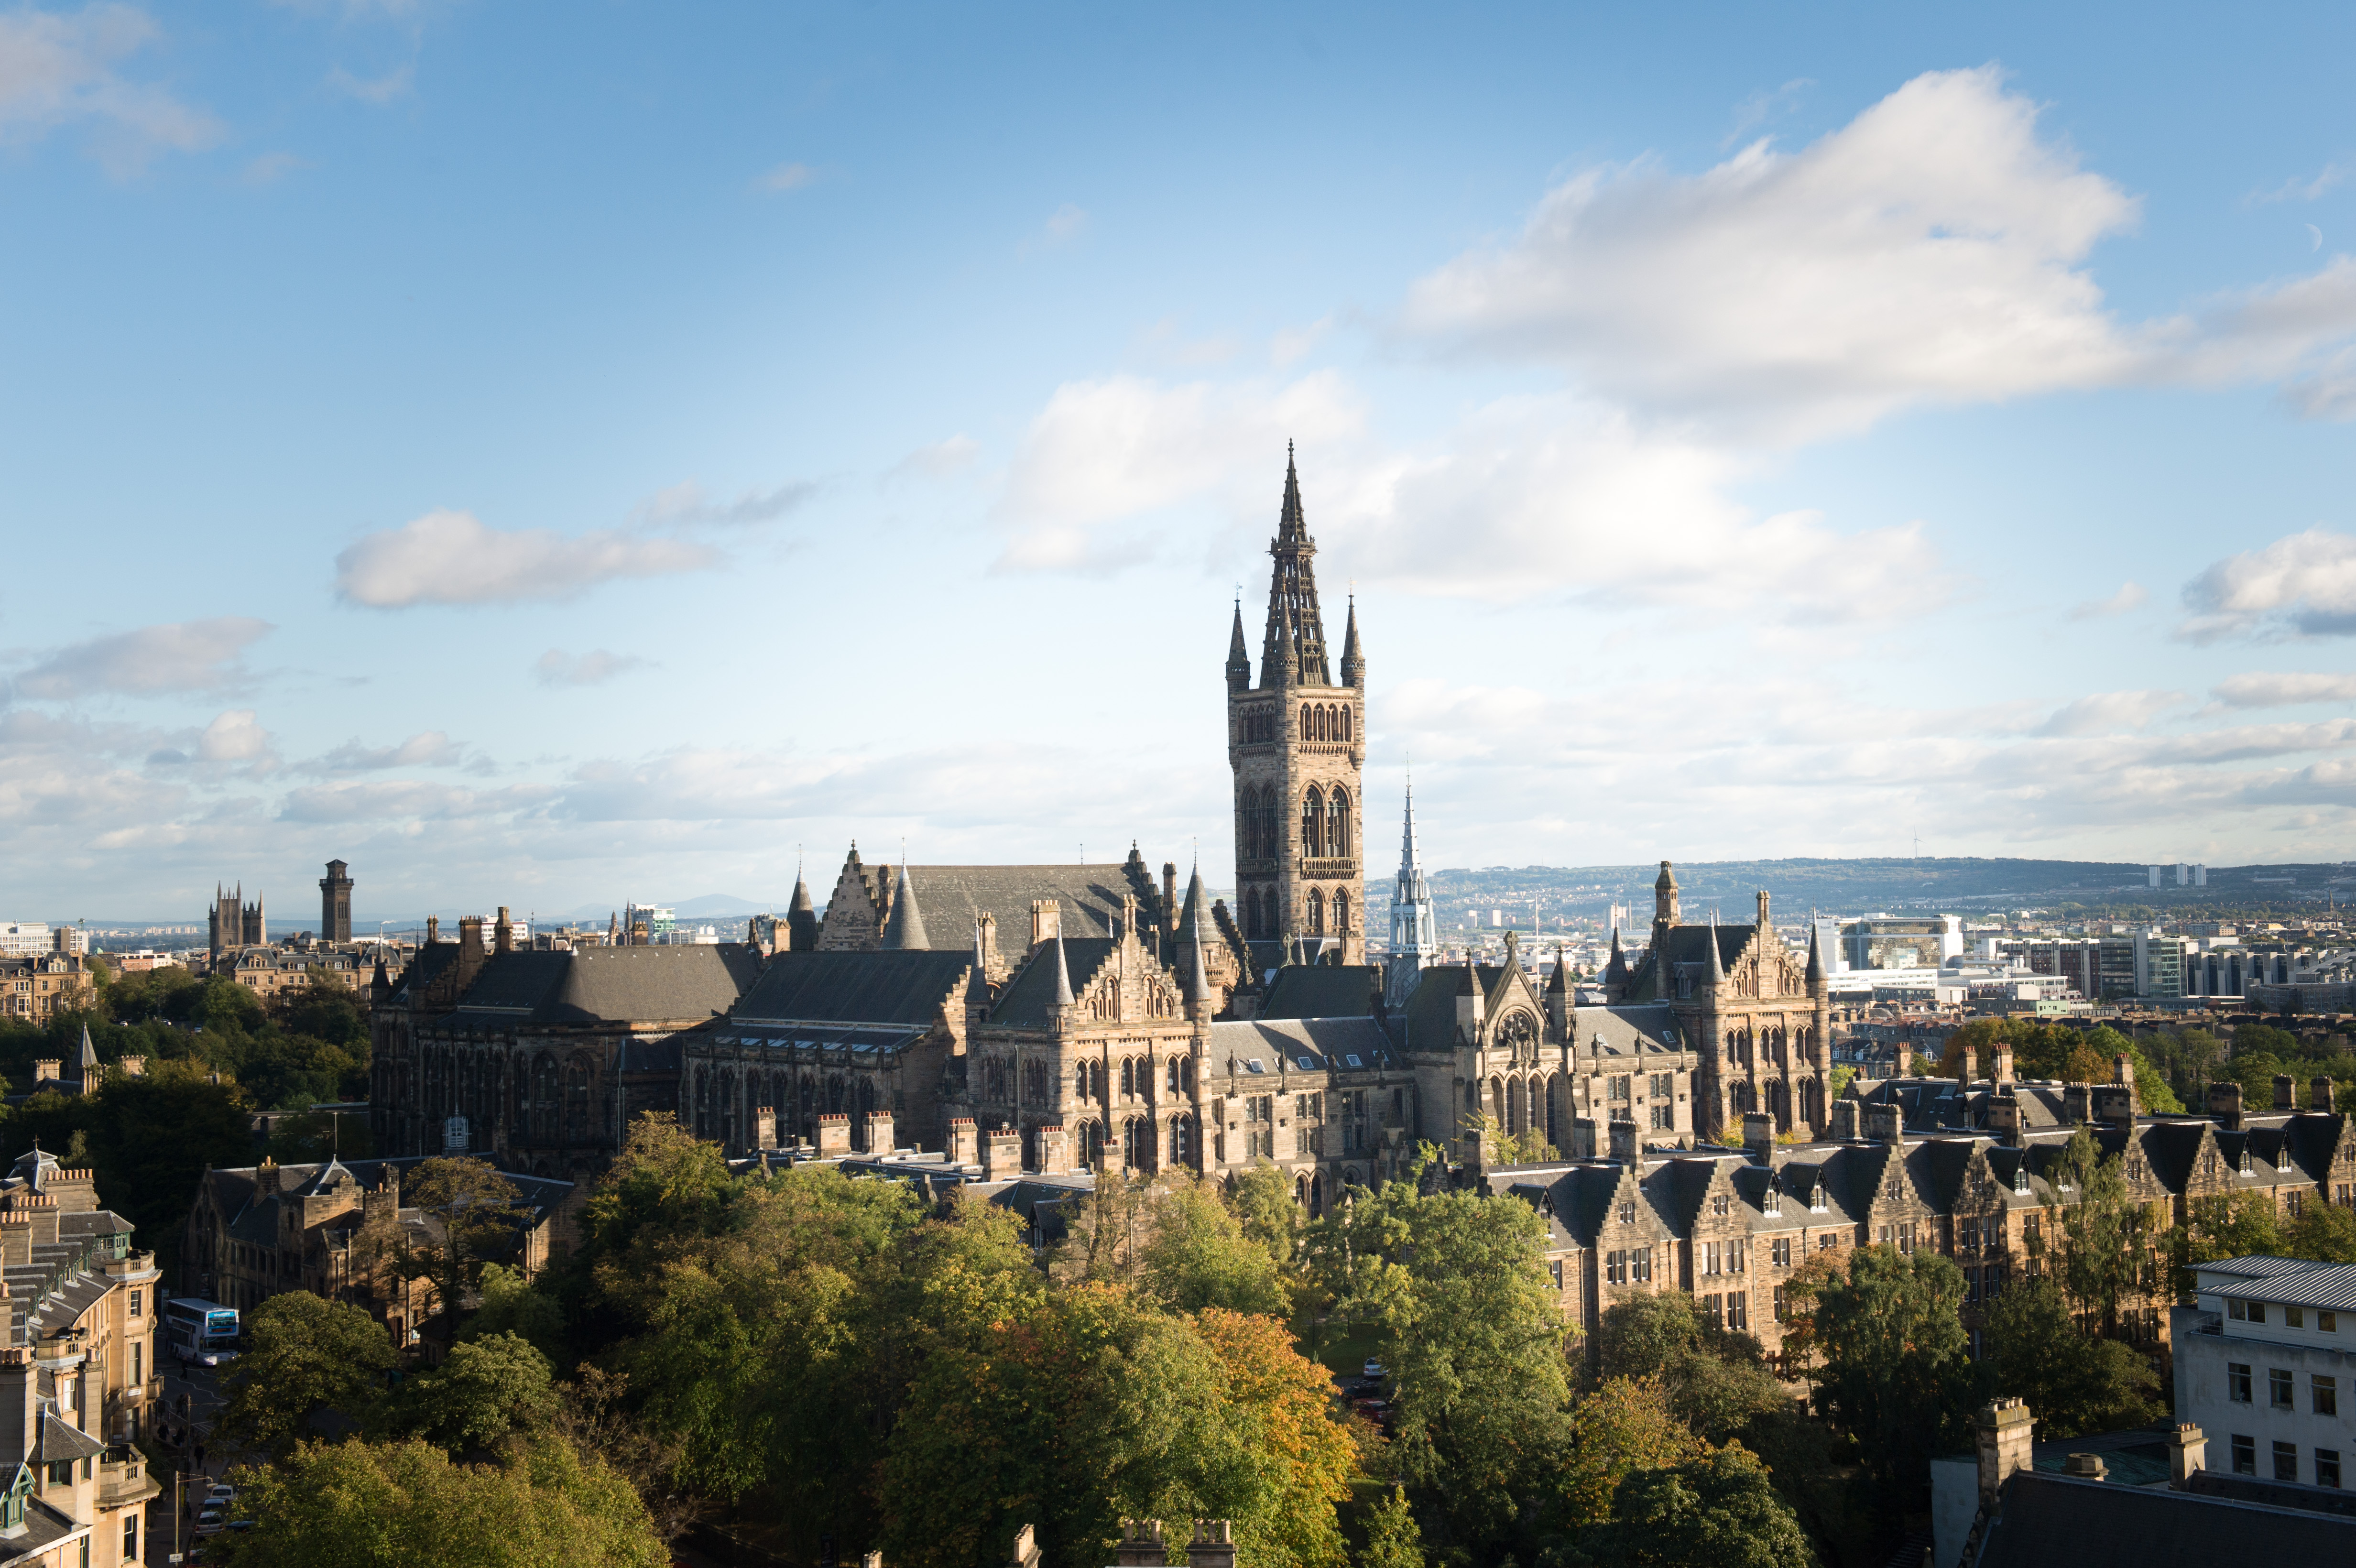
\includegraphics[keepaspectratio=true, width=\paperwidth]{../../images/background.jpg}};
    }
    \begin{frame}[plain,noframenumbering]
        \titlepage
    \end{frame}
}

\section{Finding Subgraphs}

\begin{frame}{Subgraph Isomorphism}
    \centering
    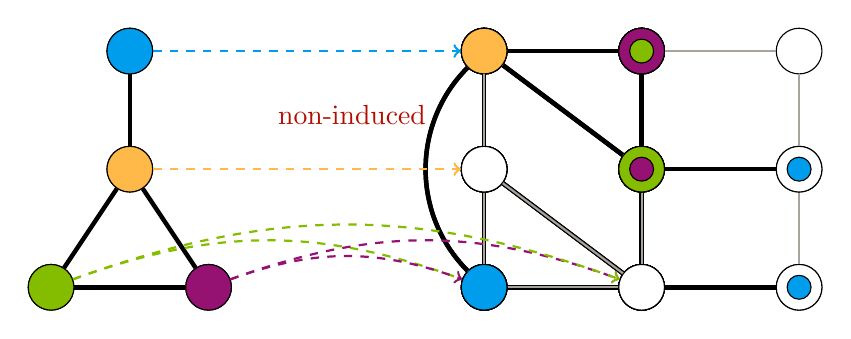
\begin{tikzpicture}
        \node <1> [draw, circle, fill=white, inner sep=4pt, font=\bfseries] (Na) at (1,  0) {\vphantom{1}};
        \node <1> [draw, circle, fill=white, inner sep=4pt, font=\bfseries] (Nb) at (1, -1.5) {\vphantom{1}};
        \node <1> [draw, circle, fill=white, inner sep=4pt, font=\bfseries] (Nc) at (0, -3) {\vphantom{1}};
        \node <1> [draw, circle, fill=white, inner sep=4pt, font=\bfseries] (Nd) at (2, -3) {\vphantom{1}};

        \node <2-> [draw, circle, fill=uofgcobalt, inner sep=4pt, font=\bfseries] (Na) at (1,  0) {\vphantom{1}};
        \node <2-> [draw, circle, fill=uofgpumpkin, inner sep=4pt, font=\bfseries] (Nb) at (1, -1.5) {\vphantom{1}};
        \node <2-> [draw, circle, fill=uofglawn, inner sep=4pt, font=\bfseries] (Nc) at (0, -3) {\vphantom{1}};
        \node <2-> [draw, circle, fill=uofgthistle, inner sep=4pt, font=\bfseries] (Nd) at (2, -3) {\vphantom{1}};

        \draw [ultra thick] (Na) -- (Nb);
        \draw [ultra thick] (Nb) -- (Nc);
        \draw [ultra thick] (Nc) -- (Nd);
        \draw [ultra thick] (Nb) -- (Nd);

        \node <1> [draw, circle, fill=white, inner sep=4pt, font=\bfseries] (N1) at (5.5,  0) {\vphantom{1}};
        \node <1> [draw, circle, fill=white, inner sep=4pt, font=\bfseries] (N2) at (7.5,  0) {\vphantom{1}};
        \node <1> [draw, circle, fill=white, inner sep=4pt, font=\bfseries] (N3) at (5.5, -1.5) {\vphantom{1}};
        \node <1> [draw, circle, fill=white, inner sep=4pt, font=\bfseries] (N4) at (7.5, -1.5) {\vphantom{1}};
        \node <1> [draw, circle, fill=white, inner sep=4pt, font=\bfseries] (N5) at (5.5, -3) {\vphantom{1}};
        \node <1> [draw, circle, fill=white, inner sep=4pt, font=\bfseries] (N6) at (7.5, -3) {\vphantom{1}};

        \node <1-6,8-> [draw, circle, fill=white, inner sep=4pt, font=\bfseries] (N7) at (9.5, -3) {\vphantom{1}};
        \node <1-4,6-> [draw, circle, fill=white, inner sep=4pt, font=\bfseries] (N8) at (9.5, -1.5) {\vphantom{1}};
        \node [draw, circle, fill=white, inner sep=4pt, font=\bfseries] (N9) at (9.5, 0) {\vphantom{1}};

        \node <2-3> [draw, circle, fill=uofgcobalt, inner sep=4pt, font=\bfseries] (N1) at (5.5,  0) {\vphantom{1}};
        \node <2-3> [draw, circle, fill=white, inner sep=4pt, font=\bfseries] (N2) at (7.5,  0) {\vphantom{1}};
        \node <2-3> [draw, circle, fill=uofgpumpkin, inner sep=4pt, font=\bfseries] (N3) at (5.5, -1.5) {\vphantom{1}};
        \node <2-3> [draw, circle, fill=white, inner sep=4pt, font=\bfseries] (N4) at (7.5, -1.5) {\vphantom{1}};
        \node <2-3> [draw, circle, fill=uofglawn, inner sep=4pt, font=\bfseries] (N5) at (5.5, -3) {\vphantom{1}};
        \node <2-3> [draw, circle, fill=uofgthistle, inner sep=4pt, font=\bfseries] (N6) at (7.5, -3) {\vphantom{1}};

        \node <4> [draw, circle, fill=uofgcobalt, inner sep=4pt, font=\bfseries] (N1) at (5.5,  0) {\vphantom{1}};
        \node <4> [draw, circle, fill=white, inner sep=4pt, font=\bfseries] (N2) at (7.5,  0) {\vphantom{1}};
        \node <4> [draw, circle, fill=uofgpumpkin, inner sep=4pt, font=\bfseries] (N3) at (5.5, -1.5) {\vphantom{1}};
        \node <4> [draw, circle, fill=white, inner sep=4pt, font=\bfseries] (N4) at (7.5, -1.5) {\vphantom{1}};
        \node <4> [draw, circle, fill=uofgthistle, inner sep=4pt, font=\bfseries] (N5) at (5.5, -3) {\vphantom{1}};
        \node <4> [draw, circle, fill=uofglawn, inner sep=4pt, font=\bfseries] (N6) at (7.5, -3) {\vphantom{1}};

        \node <5> [draw, circle, fill=uofglawn, inner sep=4pt, font=\bfseries] (N1) at (5.5,  0) {\vphantom{1}};
        \node <5> [draw, circle, fill=uofgthistle, inner sep=1pt, font=\bfseries] (N1b) at (5.5,  0) {\vphantom{1}};
        \node <5> [draw, circle, fill=uofgthistle, inner sep=4pt, font=\bfseries] (N2) at (7.5,  0) {\vphantom{1}};
        \node <5> [draw, circle, fill=uofglawn, inner sep=1pt, font=\bfseries] (N2b) at (7.5,  0) {\vphantom{1}};
        \node <5> [draw, circle, fill=white, inner sep=4pt, font=\bfseries] (N3) at (5.5, -1.5) {\vphantom{1}};
        \node <5> [draw, circle, fill=uofgpumpkin, inner sep=4pt, font=\bfseries] (N4) at (7.5, -1.5) {\vphantom{1}};
        \node <5> [draw, circle, fill=white, inner sep=4pt, font=\bfseries] (N5) at (5.5, -3) {\vphantom{1}};
        \node <5> [draw, circle, fill=white, inner sep=4pt, font=\bfseries] (N6) at (7.5, -3) {\vphantom{1}};
        \node <5> [draw, circle, fill=uofgcobalt, inner sep=1pt, font=\bfseries] (N6b) at (7.5, -3) {\vphantom{1}};
        \node <5> [draw, circle, fill=white, inner sep=4pt, font=\bfseries] (N8) at (9.5, -1.5) {\vphantom{1}};
        \node <5> [draw, circle, fill=uofgcobalt, inner sep=1pt, font=\bfseries] (N8b) at (9.5, -1.5) {\vphantom{1}};

        \node <6> [draw, circle, fill=uofgpumpkin, inner sep=4pt, font=\bfseries] (N1) at (5.5,  0) {\vphantom{1}};
        \node <6> [draw, circle, fill=uofgthistle, inner sep=4pt, font=\bfseries] (N2) at (7.5,  0) {\vphantom{1}};
        \node <6> [draw, circle, fill=uofglawn, inner sep=1pt, font=\bfseries] (N2b) at (7.5,  0) {\vphantom{1}};
        \node <6> [draw, circle, fill=uofgcobalt, inner sep=4pt, font=\bfseries] (N3) at (5.5, -1.5) {\vphantom{1}};
        \node <6> [draw, circle, fill=uofglawn, inner sep=4pt, font=\bfseries] (N4) at (7.5, -1.5) {\vphantom{1}};
        \node <6> [draw, circle, fill=uofgthistle, inner sep=1pt, font=\bfseries] (N4b) at (7.5, -1.5) {\vphantom{1}};
        \node <6> [draw, circle, fill=white, inner sep=4pt, font=\bfseries] (N5) at (5.5, -3) {\vphantom{1}};
        \node <6> [draw, circle, fill=white, inner sep=4pt, font=\bfseries] (N6) at (7.5, -3) {\vphantom{1}};

        \node <7> [draw, circle, fill=white, inner sep=4pt, font=\bfseries] (N1) at (5.5,  0) {\vphantom{1}};
        \node <7> [draw, circle, fill=white, inner sep=4pt, font=\bfseries] (N2) at (7.5,  0) {\vphantom{1}};
        \node <7> [draw, circle, fill=uofgthistle, inner sep=4pt, font=\bfseries] (N3) at (5.5, -1.5) {\vphantom{1}};
        \node <7> [draw, circle, fill=uofglawn, inner sep=1pt, font=\bfseries] (N3b) at (5.5, -1.5) {\vphantom{1}};
        \node <7> [draw, circle, fill=white, inner sep=4pt, font=\bfseries] (N4) at (7.5, -1.5) {\vphantom{1}};
        \node <7> [draw, circle, fill=uofgcobalt, inner sep=1pt, font=\bfseries] (N4b) at (7.5, -1.5) {\vphantom{1}};
        \node <7> [draw, circle, fill=uofglawn, inner sep=4pt, font=\bfseries] (N5) at (5.5, -3) {\vphantom{1}};
        \node <7> [draw, circle, fill=uofgthistle, inner sep=1pt, font=\bfseries] (N5b) at (5.5, -3) {\vphantom{1}};
        \node <7> [draw, circle, fill=uofgpumpkin, inner sep=4pt, font=\bfseries] (N6) at (7.5, -3) {\vphantom{1}};
        \node <7> [draw, circle, fill=white, inner sep=4pt, font=\bfseries] (N7) at (9.5, -3) {\vphantom{1}};
        \node <7> [draw, circle, fill=uofgcobalt, inner sep=1pt, font=\bfseries] (N7b) at (9.5, -3) {\vphantom{1}};

        \node <8> [draw, circle, fill=uofgcobalt, inner sep=4pt, font=\bfseries] (N1) at (5.5,  0) {\vphantom{1}};
        \node <8> [draw, circle, fill=white, inner sep=4pt, font=\bfseries] (N2) at (7.5,  0) {\vphantom{1}};
        \node <8> [draw, circle, fill=uofglawn, inner sep=4pt, font=\bfseries] (N3) at (5.5, -1.5) {\vphantom{1}};
        \node <8> [draw, circle, fill=uofgthistle, inner sep=1pt, font=\bfseries] (N3b) at (5.5, -1.5) {\vphantom{1}};
        \node <8> [draw, circle, fill=white, inner sep=4pt, font=\bfseries] (N4) at (7.5, -1.5) {\vphantom{1}};
        \node <8> [draw, circle, fill=uofgpumpkin, inner sep=4pt, font=\bfseries] (N5) at (5.5, -3) {\vphantom{1}};
        \node <8> [draw, circle, fill=uofgthistle, inner sep=4pt, font=\bfseries] (N6) at (7.5, -3) {\vphantom{1}};
        \node <8> [draw, circle, fill=uofglawn, inner sep=1pt, font=\bfseries] (N6b) at (7.5, -3) {\vphantom{1}};

        \node <9> [draw, circle, fill=uofgpumpkin, inner sep=4pt, font=\bfseries] (N1) at (5.5,  0) {\vphantom{1}};
        \node <9> [draw, circle, fill=uofgthistle, inner sep=4pt, font=\bfseries] (N2) at (7.5,  0) {\vphantom{1}};
        \node <9> [draw, circle, fill=uofglawn, inner sep=1pt, font=\bfseries] (N2b) at (7.5,  0) {\vphantom{1}};
        \node <9> [draw, circle, fill=white, inner sep=4pt, font=\bfseries] (N3) at (5.5, -1.5) {\vphantom{1}};
        \node <9> [draw, circle, fill=uofglawn, inner sep=4pt, font=\bfseries] (N4) at (7.5, -1.5) {\vphantom{1}};
        \node <9> [draw, circle, fill=uofgthistle, inner sep=1pt, font=\bfseries] (N4b) at (7.5, -1.5) {\vphantom{1}};
        \node <9> [draw, circle, fill=uofgcobalt, inner sep=4pt, font=\bfseries] (N5) at (5.5, -3) {\vphantom{1}};
        \node <9> [draw, circle, fill=white, inner sep=4pt, font=\bfseries] (N6) at (7.5, -3) {\vphantom{1}};

        \draw <1> [thick, color=uofgsandstone!50] (N1) -- (N2);
        \draw <1> [thick, color=uofgsandstone!50] (N1) -- (N3);
        \draw <1> [thick, color=uofgsandstone!50] (N1) -- (N4);
        \draw <1> [thick, color=uofgsandstone!50] (N2) -- (N4);
        \draw <1> [thick, color=uofgsandstone!50] (N3) -- (N5);
        \draw <1> [thick, color=uofgsandstone!50] (N3) -- (N6);
        \draw <1> [thick, color=uofgsandstone!50] (N4) -- (N6);
        \draw <1> [thick, color=uofgsandstone!50] (N5) -- (N6);
        \draw <1> [thick, color=uofgsandstone!50] (N1) to [in=135, out=225] (N5);

        \draw <2-4> [thick, color=uofgsandstone!50] (N1) -- (N2);
        \draw <2-4> [ultra thick] (N1) -- (N3);
        \draw <2-4> [thick, color=uofgsandstone!50] (N1) -- (N4);
        \draw <2-4> [thick, color=uofgsandstone!50] (N2) -- (N4);
        \draw <2-4> [ultra thick] (N3) -- (N5);
        \draw <2-4> [ultra thick] (N3) -- (N6);
        \draw <2-4> [thick, color=uofgsandstone!50] (N4) -- (N6);
        \draw <2-4> [ultra thick] (N5) -- (N6);
        \draw <2> [thick, color=uofgsandstone!50] (N1) to [in=135, out=225] (N5);
        \draw <3> [thick, color=uofgpillarbox] (N1) to [in=135, out=225] node [near start, left] { non-induced } (N5);
        \draw <4> [thick, color=uofgsandstone!50] (N1) to [in=135, out=225] (N5);

        \draw <5> [ultra thick] (N1) -- (N2);
        \draw <5> [thick, color=uofgsandstone!50] (N1) -- (N3);
        \draw <5> [ultra thick] (N1) -- (N4);
        \draw <5> [ultra thick] (N2) -- (N4);
        \draw <5> [thick, color=uofgsandstone!50] (N3) -- (N5);
        \draw <5> [thick, color=uofgsandstone!50] (N3) -- (N6);
        \draw <5> [ultra thick] (N4) -- (N6);
        \draw <5> [thick, color=uofgsandstone!50] (N5) -- (N6);
        \draw <5> [thick, color=uofgsandstone!50] (N1) to [in=135, out=225] (N5);

        \draw <6> [ultra thick] (N1) -- (N2);
        \draw <6> [ultra thick] (N1) -- (N3);
        \draw <6> [ultra thick] (N1) -- (N4);
        \draw <6> [ultra thick] (N2) -- (N4);
        \draw <6> [thick, color=uofgsandstone!50] (N3) -- (N5);
        \draw <6> [thick, color=uofgsandstone!50] (N3) -- (N6);
        \draw <6> [thick, color=uofgsandstone!50] (N4) -- (N6);
        \draw <6> [thick, color=uofgsandstone!50] (N5) -- (N6);
        \draw <6> [thick, color=uofgsandstone!50] (N1) to [in=135, out=225] (N5);

        \draw <7> [thick, color=uofgsandstone!50] (N1) -- (N2);
        \draw <7> [thick, color=uofgsandstone!50] (N1) -- (N3);
        \draw <7> [thick, color=uofgsandstone!50] (N1) -- (N4);
        \draw <7> [thick, color=uofgsandstone!50] (N2) -- (N4);
        \draw <7> [ultra thick] (N3) -- (N5);
        \draw <7> [ultra thick] (N3) -- (N6);
        \draw <7> [ultra thick] (N4) -- (N6);
        \draw <7> [ultra thick] (N5) -- (N6);
        \draw <7> [thick, color=uofgsandstone!50] (N1) to [in=135, out=225] (N5);

        \draw <8> [thick, color=uofgsandstone!50] (N1) -- (N2);
        \draw <8> [thick, color=uofgsandstone!50] (N1) -- (N3);
        \draw <8> [thick, color=uofgsandstone!50] (N1) -- (N4);
        \draw <8> [thick, color=uofgsandstone!50] (N2) -- (N4);
        \draw <8> [ultra thick] (N3) -- (N5);
        \draw <8> [ultra thick] (N3) -- (N6);
        \draw <8> [thick, color=uofgsandstone!50] (N4) -- (N6);
        \draw <8> [ultra thick] (N5) -- (N6);
        \draw <8> [ultra thick] (N1) to [in=135, out=225] (N5);

        \draw <9> [ultra thick] (N1) -- (N2);
        \draw <9> [thick, color=uofgsandstone!50] (N1) -- (N3);
        \draw <9> [ultra thick] (N1) -- (N4);
        \draw <9> [ultra thick] (N2) -- (N4);
        \draw <9> [thick, color=uofgsandstone!50] (N3) -- (N5);
        \draw <9> [thick, color=uofgsandstone!50] (N3) -- (N6);
        \draw <9> [thick, color=uofgsandstone!50] (N4) -- (N6);
        \draw <9> [thick, color=uofgsandstone!50] (N5) -- (N6);
        \draw <9> [ultra thick] (N1) to [in=135, out=225] (N5);

        \draw <2-3> [thick, dashed, color=uofgcobalt, arrows=->] (Na) to (N1);
        \draw <2-3> [thick, dashed, color=uofgpumpkin, arrows=->] (Nb) to (N3);
        \draw <2-3> [thick, dashed, color=uofglawn, arrows=->] (Nc) to [out=20, in=160] (N5);
        \draw <2-3> [thick, dashed, color=uofgthistle, arrows=->] (Nd) to [out=20, in=160] (N6);

        \draw <4> [thick, dashed, color=uofgcobalt, arrows=->] (Na) to (N1);
        \draw <4> [thick, dashed, color=uofgpumpkin, arrows=->] (Nb) to (N3);
        \draw <4> [thick, dashed, color=uofglawn, arrows=->] (Nc) to [out=20, in=160] (N6);
        \draw <4> [thick, dashed, color=uofgthistle, arrows=->] (Nd) to [out=20, in=160] (N5);

        \draw [thick, color=uofgsandstone!50] (N7) -- (N8);
        \draw [thick, color=uofgsandstone!50] (N8) -- (N9);
        \draw [thick, color=uofgsandstone!50] (N2) -- (N9);
        \draw <1-4,6-> [thick, color=uofgsandstone!50] (N4) -- (N8);
        \draw <5> [ultra thick] (N4) -- (N8);
        \draw <1-6,8-> [thick, color=uofgsandstone!50] (N6) -- (N7);
        \draw <7> [ultra thick] (N6) -- (N7);
    \end{tikzpicture}
\end{frame}

\begin{frame}{Maximum Common Induced Subgraph}
    \centering
    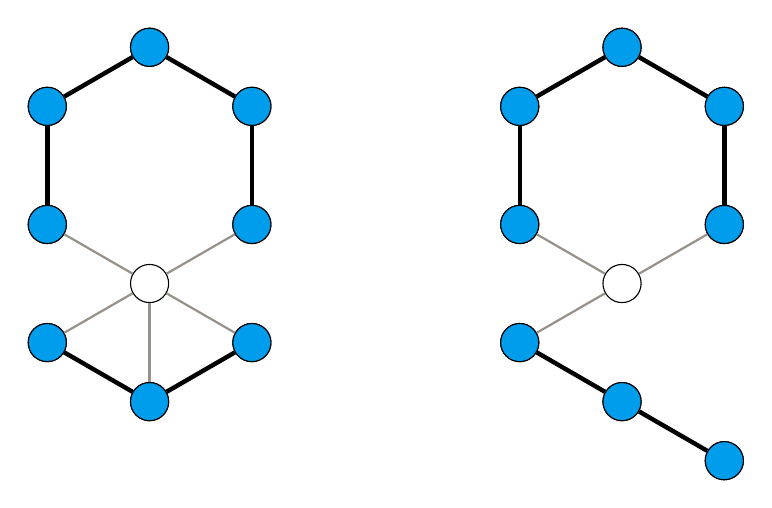
\begin{tikzpicture}
        \begin{scope}
            \node<1> [draw, circle, inner sep=2pt, font=\normalsize] (M1) at (90:1.5) {\phantom{0}};
            \node<2> [draw, circle, fill=uofgcobalt, inner sep=2pt, font=\normalsize] (M1) at (90:1.5) {\phantom{0}};
            \node<1> [draw, circle, inner sep=2pt, font=\normalsize] (M2) at (150:1.5) {\phantom{0}};
            \node<2> [draw, circle, fill=uofgcobalt, inner sep=2pt, font=\normalsize] (M2) at (150:1.5) {\phantom{0}};
            \node<1> [draw, circle, inner sep=2pt, font=\normalsize] (M3) at (30:1.5) {\phantom{0}};
            \node<2> [draw, circle, fill=uofgcobalt, inner sep=2pt, font=\normalsize] (M3) at (30:1.5) {\phantom{0}};
            \node<1> [draw, circle, inner sep=2pt, font=\normalsize] (M4) at (210:1.5) {\phantom{0}};
            \node<2> [draw, circle, fill=uofgcobalt, inner sep=2pt, font=\normalsize] (M4) at (210:1.5) {\phantom{0}};
            \node<1> [draw, circle, inner sep=2pt, font=\normalsize] (M5) at (330:1.5) {\phantom{0}};
            \node<2> [draw, circle, fill=uofgcobalt, inner sep=2pt, font=\normalsize] (M5) at (330:1.5) {\phantom{0}};
            \node[draw, circle, fill=white, inner sep=2pt, font=\normalsize] (M6) at (270:1.5) {\phantom{0}};
            \node<1> [draw, circle, inner sep=2pt, font=\normalsize] (M7) at ($(210:1.5) + (M6)$) {\phantom{0}};
            \node<2> [draw, circle, fill=uofgcobalt, inner sep=2pt, font=\normalsize] (M7) at ($(210:1.5) + (M6)$) {\phantom{0}};
            \node<1> [draw, circle, inner sep=2pt, font=\normalsize] (M8) at ($(330:1.5) + (M6)$) {\phantom{0}};
            \node<2> [draw, circle, fill=uofgcobalt, inner sep=2pt, font=\normalsize] (M8) at ($(330:1.5) + (M6)$) {\phantom{0}};
            \node<1> [draw, circle, inner sep=2pt, font=\normalsize] (M9) at ($(270:1.5) + (M6)$) {\phantom{0}};
            \node<2> [draw, circle, fill=uofgcobalt, inner sep=2pt, font=\normalsize] (M9) at ($(270:1.5) + (M6)$) {\phantom{0}};

            \draw<1> [thick, color=uofgsandstone!60] (M1) -- (M2);
            \draw<2> [ultra thick] (M1) -- (M2);
            \draw<1> [thick, color=uofgsandstone!60] (M2) -- (M4);
            \draw<2> [ultra thick] (M2) -- (M4);
            \draw<1> [thick, color=uofgsandstone!60] (M3) -- (M5);
            \draw<2> [ultra thick] (M3) -- (M5);
            \draw [thick, color=uofgsandstone!60] (M4) -- (M6);
            \draw [thick, color=uofgsandstone!60] (M5) -- (M6);
            \draw<1> [thick, color=uofgsandstone!60] (M3) -- (M1);
            \draw<2> [ultra thick] (M3) -- (M1);
            \draw [thick, color=uofgsandstone!60] (M6) -- (M7);
            \draw [thick, color=uofgsandstone!60] (M6) -- (M8);
            \draw [thick, color=uofgsandstone!60] (M6) -- (M9);
            \draw<1> [thick, color=uofgsandstone!60] (M7) -- (M9);
            \draw<2> [ultra thick] (M7) -- (M9);
            \draw<1> [thick, color=uofgsandstone!60] (M8) -- (M9);
            \draw<2> [ultra thick] (M8) -- (M9);
        \end{scope}

        \begin{scope}[xshift=6cm]
            \node<1> [draw, circle, inner sep=2pt, font=\normalsize] (M1) at (90:1.5) {\phantom{0}};
            \node<2> [draw, circle, fill=uofgcobalt, inner sep=2pt, font=\normalsize] (M1) at (90:1.5) {\phantom{0}};
            \node<1> [draw, circle, inner sep=2pt, font=\normalsize] (M2) at (150:1.5) {\phantom{0}};
            \node<2> [draw, circle, fill=uofgcobalt, inner sep=2pt, font=\normalsize] (M2) at (150:1.5) {\phantom{0}};
            \node<1> [draw, circle, inner sep=2pt, font=\normalsize] (M3) at (30:1.5) {\phantom{0}};
            \node<2> [draw, circle, fill=uofgcobalt, inner sep=2pt, font=\normalsize] (M3) at (30:1.5) {\phantom{0}};
            \node<1> [draw, circle, inner sep=2pt, font=\normalsize] (M4) at (210:1.5) {\phantom{0}};
            \node<2> [draw, circle, fill=uofgcobalt, inner sep=2pt, font=\normalsize] (M4) at (210:1.5) {\phantom{0}};
            \node<1> [draw, circle, inner sep=2pt, font=\normalsize] (M5) at (330:1.5) {\phantom{0}};
            \node<2> [draw, circle, fill=uofgcobalt, inner sep=2pt, font=\normalsize] (M5) at (330:1.5) {\phantom{0}};
            \node[draw, circle, fill=white, inner sep=2pt, font=\normalsize] (M6) at (270:1.5) {\phantom{0}};
            \node<1> [draw, circle, inner sep=2pt, font=\normalsize] (M7) at ($(210:1.5) + (M6)$) {\phantom{0}};
            \node<2> [draw, circle, fill=uofgcobalt, inner sep=2pt, font=\normalsize] (M7) at ($(210:1.5) + (M6)$) {\phantom{0}};
            \node<1> [draw, circle, inner sep=2pt, font=\normalsize] (M8) at ($(270:1.5) + (M6)$) {\phantom{0}};
            \node<2> [draw, circle, fill=uofgcobalt, inner sep=2pt, font=\normalsize] (M8) at ($(270:1.5) + (M6)$) {\phantom{0}};
            \node<1> [draw, circle, inner sep=2pt, font=\normalsize] (M9) at ($(330:1.5) + (M8)$) {\phantom{0}};
            \node<2> [draw, circle, fill=uofgcobalt, inner sep=2pt, font=\normalsize] (M9) at ($(330:1.5) + (M8)$) {\phantom{0}};

            \draw<1> [thick, color=uofgsandstone!60] (M1) -- (M2);
            \draw<2> [ultra thick] (M1) -- (M2);
            \draw<1> [thick, color=uofgsandstone!60] (M2) -- (M4);
            \draw<2> [ultra thick] (M2) -- (M4);
            \draw<1> [thick, color=uofgsandstone!60] (M3) -- (M5);
            \draw<2> [ultra thick] (M3) -- (M5);
            \draw [thick, color=uofgsandstone!60] (M4) -- (M6);
            \draw [thick, color=uofgsandstone!60] (M5) -- (M6);
            \draw<1> [thick, color=uofgsandstone!60] (M3) -- (M1);
            \draw<2> [ultra thick] (M3) -- (M1);
            \draw [thick, color=uofgsandstone!60] (M6) -- (M7);
            \draw<1> [thick, color=uofgsandstone!60] (M7) -- (M8);
            \draw<2> [ultra thick] (M7) -- (M8);
            \draw<1> [thick, color=uofgsandstone!60] (M8) -- (M9);
            \draw<2> [ultra thick] (M8) -- (M9);
        \end{scope}
    \end{tikzpicture}
\end{frame}

\begin{frame}{Maximum Common Induced Connected Subgraph}
    \centering
    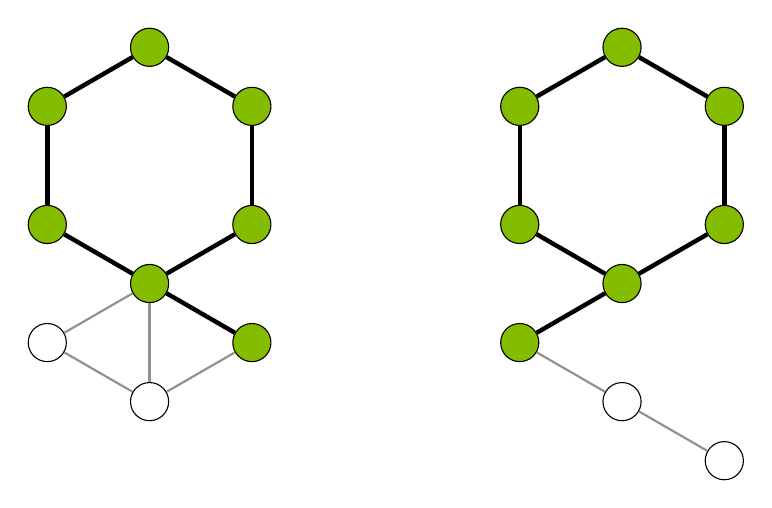
\begin{tikzpicture}
        \begin{scope}
            \node[draw, circle, fill=uofglawn, inner sep=2pt, font=\normalsize] (M1) at (90:1.5) {\phantom{0}};
            \node[draw, circle, fill=uofglawn, inner sep=2pt, font=\normalsize] (M2) at (150:1.5) {\phantom{0}};
            \node[draw, circle, fill=uofglawn, inner sep=2pt, font=\normalsize] (M3) at (30:1.5) {\phantom{0}};
            \node[draw, circle, fill=uofglawn, inner sep=2pt, font=\normalsize] (M4) at (210:1.5) {\phantom{0}};
            \node[draw, circle, fill=uofglawn, inner sep=2pt, font=\normalsize] (M5) at (330:1.5) {\phantom{0}};
            \node[draw, circle, fill=uofglawn, inner sep=2pt, font=\normalsize] (M6) at (270:1.5) {\phantom{0}};
            \node[draw, circle, fill=white, inner sep=2pt, font=\normalsize] (M7) at ($(210:1.5) + (M6)$) {\phantom{0}};
            \node[draw, circle, fill=uofglawn, inner sep=2pt, font=\normalsize] (M8) at ($(330:1.5) + (M6)$) {\phantom{0}};
            \node[draw, circle, fill=white, inner sep=2pt, font=\normalsize] (M9) at ($(270:1.5) + (M6)$) {\phantom{0}};

            \draw [ultra thick] (M1) -- (M2);
            \draw [ultra thick] (M2) -- (M4);
            \draw [ultra thick] (M3) -- (M5);
            \draw [ultra thick] (M4) -- (M6);
            \draw [ultra thick] (M5) -- (M6);
            \draw [ultra thick] (M3) -- (M1);
            \draw [thick, color=uofgsandstone!60] (M6) -- (M7);
            \draw [ultra thick] (M6) -- (M8);
            \draw [thick, color=uofgsandstone!60] (M6) -- (M9);
            \draw [thick, color=uofgsandstone!60] (M7) -- (M9);
            \draw [thick, color=uofgsandstone!60] (M8) -- (M9);
        \end{scope}

        \begin{scope}[xshift=6cm]
            \node[draw, circle, fill=uofglawn, inner sep=2pt, font=\normalsize] (M1) at (90:1.5) {\phantom{0}};
            \node[draw, circle, fill=uofglawn, inner sep=2pt, font=\normalsize] (M2) at (150:1.5) {\phantom{0}};
            \node[draw, circle, fill=uofglawn, inner sep=2pt, font=\normalsize] (M3) at (30:1.5) {\phantom{0}};
            \node[draw, circle, fill=uofglawn, inner sep=2pt, font=\normalsize] (M4) at (210:1.5) {\phantom{0}};
            \node[draw, circle, fill=uofglawn, inner sep=2pt, font=\normalsize] (M5) at (330:1.5) {\phantom{0}};
            \node[draw, circle, fill=uofglawn, inner sep=2pt, font=\normalsize] (M6) at (270:1.5) {\phantom{0}};
            \node[draw, circle, fill=uofglawn, inner sep=2pt, font=\normalsize] (M7) at ($(210:1.5) + (M6)$) {\phantom{0}};
            \node[draw, circle, fill=white, inner sep=2pt, font=\normalsize] (M8) at ($(270:1.5) + (M6)$) {\phantom{0}};
            \node[draw, circle, fill=white, inner sep=2pt, font=\normalsize] (M9) at ($(330:1.5) + (M8)$) {\phantom{0}};

            \draw [ultra thick] (M1) -- (M2);
            \draw [ultra thick] (M2) -- (M4);
            \draw [ultra thick] (M3) -- (M5);
            \draw [ultra thick] (M4) -- (M6);
            \draw [ultra thick] (M5) -- (M6);
            \draw [ultra thick] (M3) -- (M1);
            \draw [ultra thick] (M6) -- (M7);
            \draw [thick, draw=uofgsandstone!60] (M7) -- (M8);
            \draw [thick, draw=uofgsandstone!60] (M8) -- (M9);
        \end{scope}
    \end{tikzpicture}
\end{frame}

\begin{frame}{Maximum Clique}
    \centering
    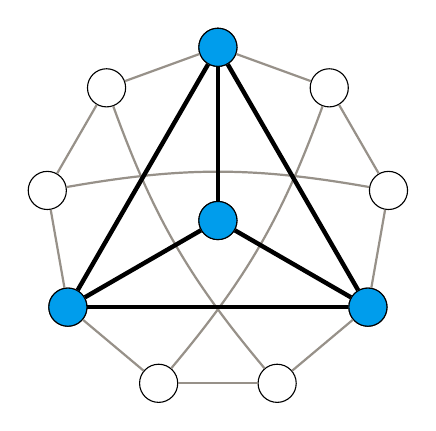
\begin{tikzpicture}
        \newcount \myc
        \foreach \n in {1, ..., 9}{
            \myc=\n \advance\myc by -1 \multiply\myc by -360 \divide\myc by 9 \advance\myc by 290
            \ifthenelse{\n = 3 \OR \n = 6 \OR \n = 9}{
                \node<1>[draw, circle, inner sep=2pt] (N\n) at (\the\myc:2.2) {\phantom{0}};
                \node<2>[draw, circle, fill=uofgcobalt, inner sep=2pt] (N\n) at (\the\myc:2.2) {\phantom{0}};
            }{
                \node[draw, circle, fill=white, inner sep=2pt] (N\n) at (\the\myc:2.2) {\phantom{0}};
            }
        }
        \node<1>[draw, circle, inner sep=2pt] (N10) at (0, 0) {\phantom{0}};
        \node<2>[draw, circle, fill=uofgcobalt, inner sep=2pt] (N10) at (0, 0) {\phantom{0}};

        \draw [thick, color=uofgsandstone!60] (N1) -- (N2);
        \draw [thick, color=uofgsandstone!60] (N2) -- (N3);
        \draw [thick, color=uofgsandstone!60] (N3) -- (N4);
        \draw [thick, color=uofgsandstone!60] (N4) -- (N5);
        \draw [thick, color=uofgsandstone!60] (N5) -- (N6);
        \draw [thick, color=uofgsandstone!60] (N6) -- (N7);
        \draw [thick, color=uofgsandstone!60] (N7) -- (N8);
        \draw [thick, color=uofgsandstone!60] (N8) -- (N9);
        \draw [thick, color=uofgsandstone!60] (N9) -- (N1);

        \draw [thick, color=uofgsandstone!60] (N4) to [out=10, in=170] (N8);
        \draw [thick, color=uofgsandstone!60] (N2) to [out=50, in=250] (N7);
        \draw [thick, color=uofgsandstone!60] (N5) to [out=290, in=130] (N1);

        \draw<1> [thick, color=uofgsandstone!60] (N3) -- (N10);
        \draw<2> [ultra thick] (N3) -- (N10);
        \draw<1> [thick, color=uofgsandstone!60] (N6) -- (N10);
        \draw<2> [ultra thick] (N6) -- (N10);
        \draw<1> [thick, color=uofgsandstone!60] (N9) -- (N10);
        \draw<2> [ultra thick] (N9) -- (N10);
        \draw<1> [thick, color=uofgsandstone!60] (N6) -- (N3);
        \draw<2> [ultra thick] (N6) -- (N3);
        \draw<1> [thick, color=uofgsandstone!60] (N9) -- (N3);
        \draw<2> [ultra thick] (N9) -- (N3);
        \draw<1> [thick, color=uofgsandstone!60] (N6) -- (N9);
        \draw<2> [ultra thick] (N6) -- (N9);
    \end{tikzpicture}
\end{frame}

\begin{frame}{Who Cares?}
    \begin{itemize}
        \item Chemistry, biochemistry, and drug design (graphs are molecule fragments or proteins).
        \item Computer vision.
        \item Compilers (instruction generation, code rewriting).
        \item Plagiarism and malware detection.
        \item Livestock epidemiology (contact and trade graphs).
        \item Designing mechanical lock systems.
    \end{itemize}
\end{frame}

\begin{frame}{In Theory\ldots}
    \begin{itemize}
        \item Subgraph finding is hard.
        \item Subgraph counting is hard.
        \item Approximate subgraph finding is hard.
    \end{itemize}
\end{frame}

\begin{frame}{In Practice\ldots}
    \begin{itemize}
        \item We have good \emph{solvers} for subgraph problems.
        \item Some applications involve solving thousands of subgraph isomorphism queries per second.
        \item We can solve clique on larger graphs than we can solve all-pairs
            shortest path.\footnote{Terms and conditions apply.}
        \item<2-> Maximum common subgraph is still a nightmare\ldots
        \item<3-> People often don't actually want to solve simple subgraph isomorphism.
    \end{itemize}
\end{frame}

\begin{frame}{Graphs Aren't Just Graphs}
    \begin{itemize}
        \item Vertex and / or edge labels, or broader compatibility functions.
        \item Directed edges.
        \item Multi-edges, more than one edge between vertices.
        \item Hyper-edges, between more than two vertices.
        \item Partially defined graphs?
        \item No need for injectivity (homomorphism), or only local injectivity.
        \item <2-> Don't forget about loops!
        \item <3-> Might want all solutions, or a count.
    \end{itemize}
\end{frame}

\section{Algorithm Basics}

\begin{frame}{Two Solver Design Philosophies}
    \begin{enumerate}
        \item Pick a vertex, guess where it goes, and start trying to grow a connected component.
            \begin{itemize}
                \item Popular solvers: VF2, VF3, RI, TurboISO, \ldots
                \item Very fast to start up.
                \item Often good on easy instances.
                \item Spectacularly bad on hard instances, and on some easy instances.
            \end{itemize}
        \item Use constraint programming, build a mapping from the pattern graph to the target
            graph.
            \begin{itemize}
                \item LAD, Glasgow Subgraph Solver.
                \item Consistent performance on easy instances.
                \item Much better on hard instances.
            \end{itemize}
    \end{enumerate}
\end{frame}

\begin{frame}{The Glasgow Subgraph Solver}
    \begin{center}
        \url{https://github.com/ciaranm/glasgow-subgraph-solver}
    \end{center}

    \begin{itemize}
        \item A CP style solver specifically for subgraph algorithms.
        \item Subgraph isomorphism, and all its variants (induced / non-induced, homomorphism,
            locally injective, labels, side constraints, directed, \ldots).
        \item Also special algorithms for clique.
        \item Guaranteed no bugs!
            \begin{itemize}
                \item<2-> Or at least, any buggy output will always be detected, if you enable proof
                    logging.
            \end{itemize}
    \end{itemize}
\end{frame}

\begin{frame}{Benchmark Instances}
    \begin{center}
        \url{http://perso.citi-lab.fr/csolnon/SIP.html}
    \end{center}

    \begin{itemize}
        \item 14,621 instances from Christine Solnon's collection:
            \begin{itemize}
                \item Randomly generated with different models (MIVIA suite).
                \item Real-world graphs.
                \item Computer vision problems.
                \item Biochemistry problems.
                \item Phase transition instances.
            \end{itemize}
        \item At least\ldots
            \begin{itemize}
                \item $\ge$ 2,110 satisfiable.
                \item $\ge$ 12,322 unsatisfiable.
            \end{itemize}
        \item A lot of them are very easy for good algorithms.
    \end{itemize}
\end{frame}

\begin{frame}{Is It Any Good?}

    \centering
    \includegraphics<1>{gen-graph-others.pdf}%

\end{frame}

\begin{frame}{Easy Conclusion!}
    \begin{itemize}
        \item CP is best!
    \end{itemize}
\end{frame}

\begin{frame}{An Observation about Certain Datasets}
    \begin{itemize}
        \item All of the randomly generated instances from the MIVIA suites are satisfiable.
        \item The target graphs are randomly generated, and patterns are made by selecting
            random connected subgraphs and permuting them.
        \item These instances are usually rather easy\ldots
        \item Many papers use \emph{only} these instances for benchmarking.
    \end{itemize}
\end{frame}

\begin{frame}{A Different Easy Conclusion!}
    \begin{itemize}
        \item CP is slow! RI is best!
    \end{itemize}
\end{frame}

\begin{frame}{Constraint Programming}
    \begin{itemize}
        \item We have some \textcolor{uofgcobalt}{variables}, each of which has a
            \textcolor{uofgcobalt}{domain} of possible \textcolor{uofgcobalt}{values}.
        \item Give each variable a value from its domain, whilst respecting all
            \textcolor{uofgcobalt}{constraints}.
    \end{itemize}
\end{frame}

\begin{frame}{Building a Mapping}
    \begin{itemize}
        \item One variable per pattern vertex.
        \item Domains and values are target vertices.
        \item We think of these variables as defining a function.
    \end{itemize}
\end{frame}

\begin{frame}{Injectivity}
    \begin{itemize}
        \item Can't map to the same target vertex twice.
        \item Could say that each pair of pattern vertices are not equal?
        \item <2-> We prefer high-level constraints, so we just say ``all different''.
    \end{itemize}
\end{frame}

\begin{frame}{Adjacency}
    \begin{itemize}
        \item If A and B are adjacent in the pattern, $f(A)$ must be adjacent to $f(B)$
            in the target.
        \item Various ways of encoding this. In SAT we'd need $n^4$ clauses, or $n^3$ if
            we're sneaky.
        \item In practice: we write a special constraint propagator to do this efficiently.
    \end{itemize}
\end{frame}

\begin{frame}{Backtracking Search, Maintaining Consistency}
    \begin{itemize}
        \item Pick a variable $V$ that has more than one value remaining.
        \item For each of its values $v$ in turn:
            \begin{itemize}
                \item Try $V = v$, and do some inference.
                    \begin{itemize}
                        \item No other variable can take the value $v$.
                        \item Variables adjacent to $V$ must be given values adjacent to $v$.
                    \end{itemize}
                \item If we get an empty domain, we made a bad guess.
                \item If every variable has one value left, we have a solution.
                \item Otherwise, recurse.
            \end{itemize}
    \end{itemize}
\end{frame}

\begin{frame}{Data Structures}
    \begin{itemize}
        \item We store a set of values for every variable.
        \item Need to be able to test whether a specific value is present, remove values,
            count how many values remain.
        \item Must either be copyable, or have some way of doing backtracking.
        \item <2-> Objectively correct answer: bitsets.
    \end{itemize}
\end{frame}

\section{Filtering}

\begin{frame}{Degree Filtering}
    \begin{itemize}
        \item Can't map a vertex of degree $d$ to a vertex of degree less than $d$.
    \end{itemize}

    \bigskip

    \centering
    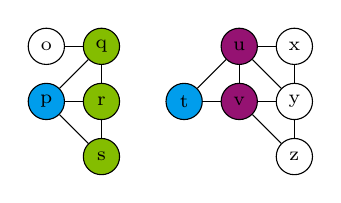
\begin{tikzpicture}
        \node [draw, circle, fill=white, inner sep=2.5pt, font=\scriptsize] (NO) at (0, 0.7) {\phantom{1}};
        \node [anchor=center, font=\scriptsize] at (NO) {o};
        \node [draw, circle, fill=uofgcobalt, inner sep=2.5pt, font=\scriptsize] (NP) at (0, 0) {\phantom{1}};
        \node [anchor=center, font=\scriptsize] at (NP) {p};
        \node [draw, circle, fill=uofglawn, inner sep=2.5pt, font=\scriptsize] (NQ) at (0.7, 0.7) {\phantom{1}};
        \node [anchor=center, font=\scriptsize] at (NQ) {q};
        \node [draw, circle, fill=uofglawn, inner sep=2.5pt, font=\scriptsize] (NR) at (0.7, 0) {\phantom{1}};
        \node [anchor=center, font=\scriptsize] at (NR) {r};
        \node [draw, circle, fill=uofglawn, inner sep=2.5pt, font=\scriptsize] (NS) at (0.7, -0.7) {\phantom{1}};
        \node [anchor=center, font=\scriptsize] at (NS) {s};
        \draw (NO) -- (NQ);
        \draw (NP) -- (NQ);
        \draw (NP) -- (NR);
        \draw (NP) -- (NS);
        \draw (NQ) -- (NR);
        \draw (NR) -- (NS);

        \node [draw, circle, fill=uofgcobalt, inner sep=2.5pt, font=\scriptsize] (NT) at (1.75, 0) {\phantom{1}};
        \node [anchor=center, font=\scriptsize] at (NT) {t};
        \node [draw, circle, fill=uofgthistle, inner sep=2.5pt, font=\scriptsize] (NU) at (2.45, 0.7) {\phantom{1}};
        \node [anchor=center, font=\scriptsize] at (NU) {u};
        \node [draw, circle, fill=uofgthistle, inner sep=2.5pt, font=\scriptsize] (NV) at (2.45, 0) {\phantom{1}};
        \node [anchor=center, font=\scriptsize] at (NV) {v};
        \node [draw, circle, fill=white, inner sep=2.5pt, font=\scriptsize] (NX) at (3.15, 0.7) {\phantom{1}};
        \node [anchor=center, font=\scriptsize] at (NX) {x};
        \node [draw, circle, fill=white, inner sep=2.5pt, font=\scriptsize] (NY) at (3.15, 0) {\phantom{1}};
        \node [anchor=center, font=\scriptsize] at (NY) {y};
        \node [draw, circle, fill=white, inner sep=2.5pt, font=\scriptsize] (NZ) at (3.15, -0.7) {\phantom{1}};
        \node [anchor=center, font=\scriptsize] at (NZ) {z};
        \draw (NT) -- (NU);
        \draw (NT) -- (NV);
        \draw (NU) -- (NV);
        \draw (NU) -- (NX);
        \draw (NU) -- (NY);
        \draw (NV) -- (NY);
        \draw (NX) -- (NY);
        \draw (NY) -- (NZ);
        \draw (NV) -- (NZ);
    \end{tikzpicture}
\end{frame}

\begin{frame}{Neighbourhood Degree Sequences}
    \begin{itemize}
        \item Can't map a vertex whose neighbours have degree 4, 3, 2 to a vertex whose neighbours
            have degree 4, 2, 2, 2.
    \end{itemize}
\end{frame}

\begin{frame}{Dynamic Degrees?}
    \begin{itemize}
        \item If a target vertex disappears from every domain, can pretend it's not there at all.
        \item This reduces the degree of all of its neighbours.
        \item Maybe this leads to more filtering?
        \item <2-> Problem: detecting this can be moderately expensive, so possibly not worth doing?
    \end{itemize}
\end{frame}

\begin{frame}{Adjacency Filtering}
    \begin{itemize}
        \item When $P$ gets mapped to $t$, neighbours of $P$ can only be mapped to neighbours
            of $t$.
        \item Store domains and neighbourhoods as bitsets.
    \end{itemize}
\end{frame}

\begin{frame}{Injectivity Filtering}
    \begin{align*}
        A &\in \{ 1, 2 \} \\
        B &\in \{ 2, 3 \} \\
        C &\in \{ 1, 3 \} \\
        D &\in \{ 1, 4, 5, 6 \} \\
        E &\in \{ 2, 5 \} \\
        F &\in \{ 3, 5 \}
    \end{align*}
\end{frame}

\begin{frame}{Matchings and All-Different}
    \begin{columns}
        \begin{column}{0.76\textwidth}
            \begin{itemize}
                \item Draw a vertex on the left for each variable, and a vertex on the right for each value.
                \item Draw edges from each variable to each of its values.
                \item A \emph{maximum cardinality matching} is where you pick as many edges as
                    possible, but each vertex can only be used at most once.
                \item We can find this in polynomial time.
                \item There is a matching which covers each variable if and only if the constraint
                    can be satisfied.
                \item In fact, there is a one to one correspondence between
                    perfect matchings and solutions to the constraint.
            \end{itemize}
        \end{column}
        \begin{column}{0.22\textwidth}
            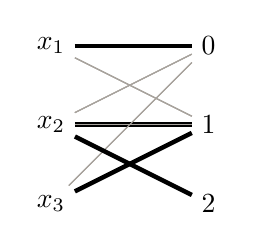
\begin{tikzpicture}
                \node (X1) at (0, 2) { $x_1$ };
                \node (X2) at (0, 1) { $x_2$ };
                \node (X3) at (0, 0) { $x_3$ };

                \node (V0) at (2, 2) { $0$ };
                \node (V1) at (2, 1) { $1$ };
                \node <3-> (V2) at (2, 0) { $2$ };

                \draw <1, 3> [color=uofgsandstone!50] (X1) -- (V0);
                \draw <1, 3> [color=uofgsandstone!50] (X1) -- (V1);
                \draw <1, 3> [color=uofgsandstone!50] (X2) -- (V0);
                \draw <1, 3> [color=uofgsandstone!50] (X2) -- (V1);
                \draw <1, 3> [color=uofgsandstone!50] (X3) -- (V0);
                \draw <1, 3> [color=uofgsandstone!50] (X3) -- (V1);
                \draw <3> [color=uofgsandstone!50] (X2) -- (V2);

                \draw <2> [color=uofgsandstone!50] (X1) -- (V1);
                \draw <2> [color=uofgsandstone!50] (X2) -- (V0);
                \draw <2> [color=uofgsandstone!50] (X3) -- (V0);
                \draw <2> [color=uofgsandstone!50] (X3) -- (V1);
                \draw <2> [ultra thick] (X1) -- (V0);
                \draw <2> [ultra thick] (X2) -- (V1);

                \draw <4> [color=uofgsandstone!50] (X1) -- (V1);
                \draw <4> [color=uofgsandstone!50] (X2) -- (V0);
                \draw <4> [color=uofgsandstone!50] (X2) -- (V1);
                \draw <4> [color=uofgsandstone!50] (X3) -- (V0);
                \draw <4> [ultra thick] (X1) -- (V0);
                \draw <4> [ultra thick] (X3) -- (V1);
                \draw <4> [ultra thick] (X2) -- (V2);
            \end{tikzpicture}
        \end{column}
    \end{columns}
\end{frame}

\begin{frame}{Sudoku}

    \centering
    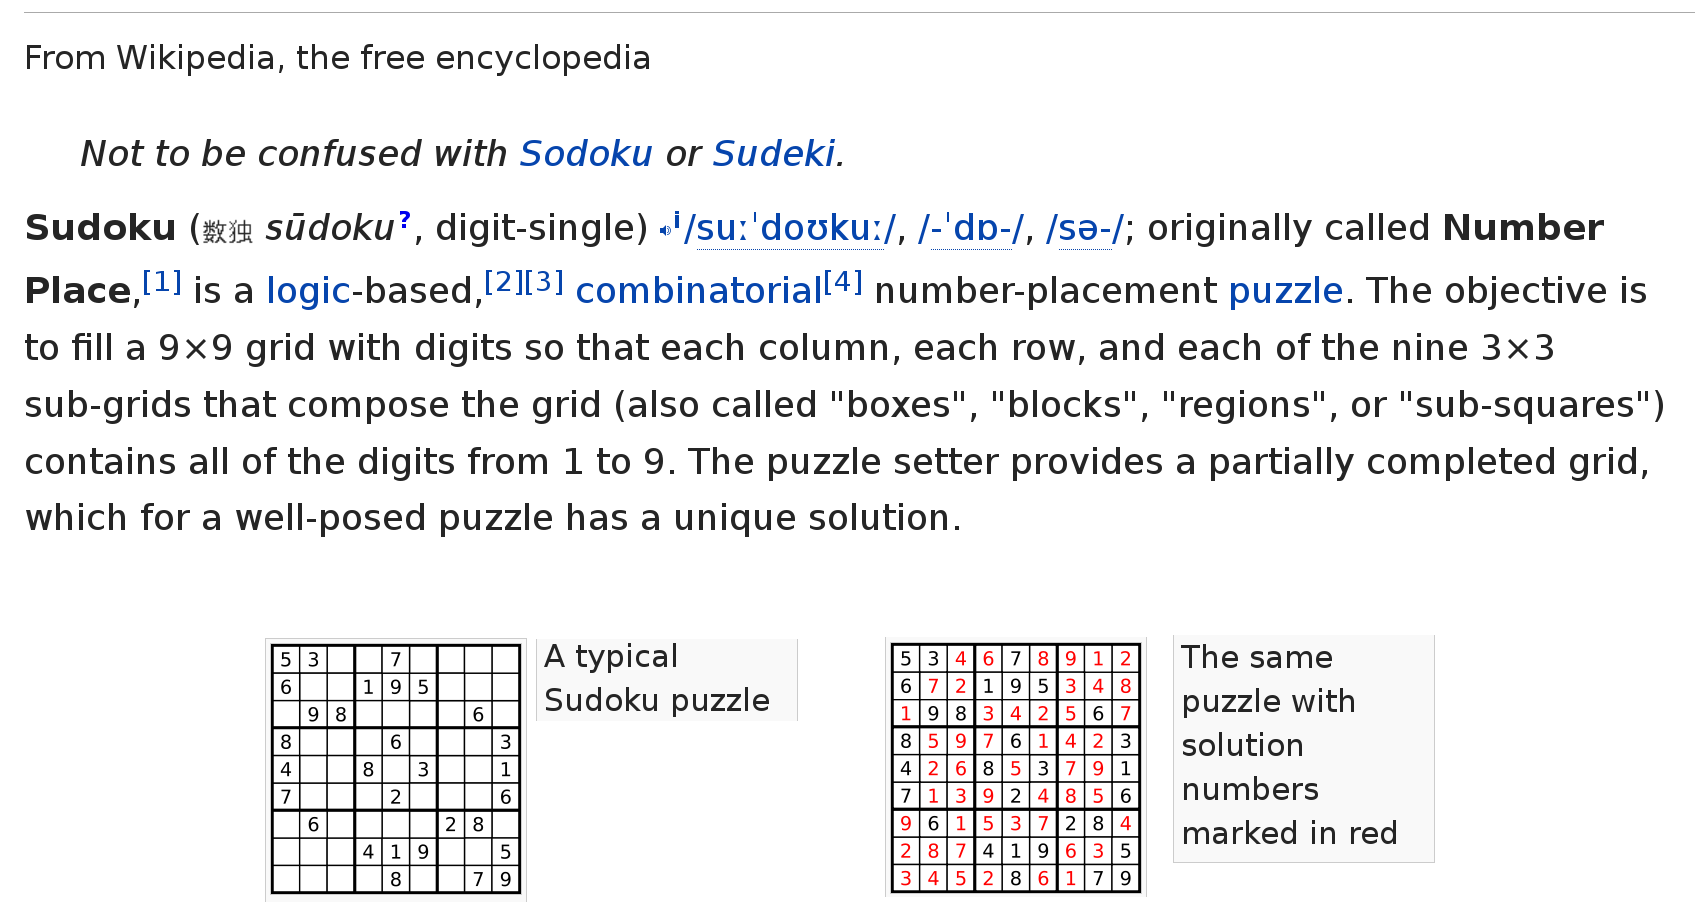
\includegraphics[keepaspectratio=true,scale=0.18]{sudoku.png}

\end{frame}

\begin{frame}{How do Humans Solve Sudoku?}
    \begin{center}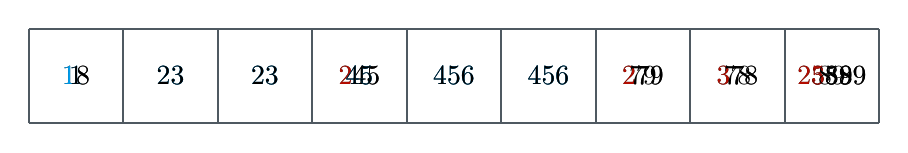
\begin{tikzpicture}[scale=0.4]
        \draw[thick, scale=3, color=uofgslate] (0, 0) grid (9, 1);

        \node <1>   [anchor=center] at (1.5, 1.5)  { 18 };
        \node <2>   [anchor=center] at (1.5, 1.5)  { \textcolor{uofgcobalt}{1}8 };
        \node <3>   [anchor=center] at (1.5, 1.5)  { \textcolor{uofgcobalt}{1} };
        \node <4->  [anchor=center] at (1.5, 1.5)  { 1 };

        \node <1-4> [anchor=center] at (4.5, 1.5)  { 23 };
        \node <5-6> [anchor=center] at (4.5, 1.5)  { \textcolor{uofgcobalt}{23} };
        \node <7->  [anchor=center] at (4.5, 1.5)  { 23 };

        \node <1-4> [anchor=center] at (7.5, 1.5)  { 23 };
        \node <5-6> [anchor=center] at (7.5, 1.5)  { \textcolor{uofgcobalt}{23} };
        \node <7->  [anchor=center] at (7.5, 1.5)  { 23 };

        \node <1-5> [anchor=center] at (10.5, 1.5) { 245 };
        \node <6>   [anchor=center] at (10.5, 1.5) { \textcolor{uofgpillarbox}{2}45 };
        \node <7>   [anchor=center] at (10.5, 1.5) { 45 };
        \node <8-9> [anchor=center] at (10.5, 1.5) { \textcolor{uofgcobalt}{45} };
        \node <10-> [anchor=center] at (10.5, 1.5) { 45 };

        \node <1-7> [anchor=center] at (13.5, 1.5) { 456 };
        \node <8-9>  [anchor=center] at (13.5, 1.5) { \textcolor{uofgcobalt}{456} };
        \node <10-> [anchor=center] at (13.5, 1.5) { 456 };

        \node <1-7> [anchor=center] at (16.5, 1.5) { 456 };
        \node <8-9> [anchor=center] at (16.5, 1.5) { \textcolor{uofgcobalt}{456} };
        \node <10-> [anchor=center] at (16.5, 1.5) { 456 };

        \node <1-5> [anchor=center] at (19.5, 1.5) { 279 };
        \node <6>   [anchor=center] at (19.5, 1.5) { \textcolor{uofgpillarbox}{2}79 };
        \node <7->  [anchor=center] at (19.5, 1.5) { 79 };

        \node <1-5> [anchor=center] at (22.5, 1.5) { 378 };
        \node <6>   [anchor=center] at (22.5, 1.5) { \textcolor{uofgpillarbox}{3}78 };
        \node <7->  [anchor=center] at (22.5, 1.5) { 78 };

        \node <1-5> [anchor=center] at (25.5, 1.5) { 23589 };
        \node <6>   [anchor=center] at (25.5, 1.5) { \textcolor{uofgpillarbox}{23}589 };
        \node <7-8> [anchor=center] at (25.5, 1.5) { 589 };
        \node <9>   [anchor=center] at (25.5, 1.5) { \textcolor{uofgpillarbox}{5}89 };
        \node <10-> [anchor=center] at (25.5, 1.5) { 89 };

    \end{tikzpicture}\end{center}
\end{frame}

\begin{frame}{Generalised Arc Consistency}
    \begin{itemize}
        \item Arc Consistency (AC): for a binary constraint, each value is supported by at least one
            value in the other variable.
        \item Generalised Arc Consistency (GAC): for a global constraint, we can pick any value from any
            variable, and find a supporting set of values from each other variable in the constraint
            simultaneously.
            \begin{itemize}
                \item Each remaining value appears in at least one solution to the constraint.
            \end{itemize}
    \end{itemize}
\end{frame}

\begin{frame}{Hall Sets}
    \begin{itemize}
        \item A \emph{Hall set} of size $n$ is a set of $n$ variables from an ``all different''
            constraint, whose domains have $n$ values between them.

        \item If we can find a Hall set, we can safely remove these values from the domains of every
            other variable involved in the constraint.

        \item Hall's Marriage Theorem: doing this is equivalent to deleting every edge from the
            matching graph which cannot appear in any perfect matching.

        \item So, if we delete every Hall set, we delete every value that cannot appear in at least
            one way of satisfying the constraint. In other words, we obtain GAC.
    \end{itemize}
\end{frame}

\begin{frame}{GAC for All-Different}
    \only<1> {
        \begin{itemize}
            \item There are $2^n$ potential Hall sets, so considering them all is probably a bad
                idea\ldots
            \item Similarly, enumerating every perfect matching is \#P-hard.
            \item However, there is a polynomial algorithm!
        \end{itemize}
    }

    \only <2-12> {
        \begin{tikzpicture}[remember picture, overlay]
            \node [anchor=north east, shift={(-0.4cm,-0.8cm)}] at (current page.north east) {
                \begin{tikzpicture}[scale=0.25, font=\tiny]
                    \draw[thick, scale=3, color=uofgslate] (0, 0) grid (9, 1);
                    \node <2-11> [anchor=center] at (1.5, 1.5)  { 18 };
                    \node <2-11> [anchor=center] at (4.5, 1.5)  { 23 };
                    \node <2-11> [anchor=center] at (7.5, 1.5)  { 23 };
                    \node <2-11> [anchor=center] at (10.5, 1.5) { 245 };
                    \node <2-11> [anchor=center] at (13.5, 1.5) { 456 };
                    \node <2-11> [anchor=center] at (16.5, 1.5) { 456 };
                    \node <2-11> [anchor=center] at (19.5, 1.5) { 279 };
                    \node <2-11> [anchor=center] at (22.5, 1.5) { 378 };
                    \node <2-11> [anchor=center] at (25.5, 1.5) { 23589 };

                    \node <12> [anchor=center] at (1.5, 1.5)  { \textcolor{uofgcobalt}{1}\textcolor{uofgpillarbox}{8} };
                    \node <12> [anchor=center] at (4.5, 1.5)  { 23 };
                    \node <12> [anchor=center] at (7.5, 1.5)  { 23 };
                    \node <12> [anchor=center] at (10.5, 1.5) { \textcolor{uofgpillarbox}{2}45 };
                    \node <12> [anchor=center] at (13.5, 1.5) { 456 };
                    \node <12> [anchor=center] at (16.5, 1.5) { 456 };
                    \node <12> [anchor=center] at (19.5, 1.5) { \textcolor{uofgpillarbox}{2}79 };
                    \node <12> [anchor=center] at (22.5, 1.5) { \textcolor{uofgpillarbox}{3}78 };
                    \node <12> [anchor=center] at (25.5, 1.5) { \textcolor{uofgpillarbox}{235}89 };
                \end{tikzpicture}
            };
        \end{tikzpicture}%
        \centering
        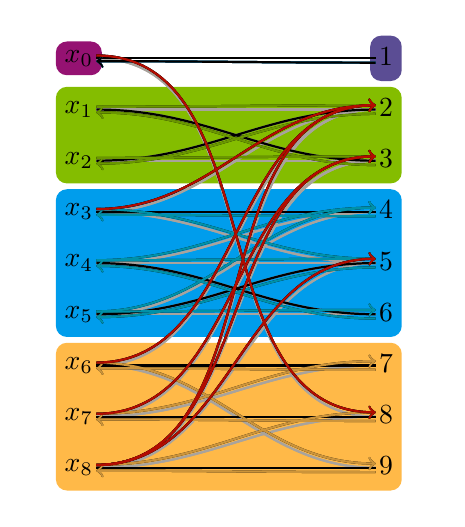
\begin{tikzpicture}[scale=0.65]
            \path (-1, -0.6) rectangle (7, 8.6);
            \node <3-> [inner sep = 1pt] (X1) at (0, 8) { $x_0$ };
            \node <3-> [inner sep = 1pt] (X2) at (0, 7) { $x_1$ };
            \node <3-> [inner sep = 1pt] (X3) at (0, 6) { $x_2$ };
            \node <3-> [inner sep = 1pt] (X4) at (0, 5) { $x_3$ };
            \node <3-> [inner sep = 1pt] (X5) at (0, 4) { $x_4$ };
            \node <3-> [inner sep = 1pt] (X6) at (0, 3) { $x_5$ };
            \node <3-> [inner sep = 1pt] (X7) at (0, 2) { $x_6$ };
            \node <3-> [inner sep = 1pt] (X8) at (0, 1) { $x_7$ };
            \node <3-> [inner sep = 1pt] (X9) at (0, 0) { $x_8$ };

            \node <4-> [inner sep = 1pt] (V1) at (6, 8) { $1\vphantom{[]}$ };
            \node <4-> [inner sep = 1pt] (V2) at (6, 7) { $2\vphantom{[]}$ };
            \node <4-> [inner sep = 1pt] (V3) at (6, 6) { $3\vphantom{[]}$ };
            \node <4-> [inner sep = 1pt] (V4) at (6, 5) { $4\vphantom{[]}$ };
            \node <4-> [inner sep = 1pt] (V5) at (6, 4) { $5\vphantom{[]}$ };
            \node <4-> [inner sep = 1pt] (V6) at (6, 3) { $6\vphantom{[]}$ };
            \node <4-> [inner sep = 1pt] (V7) at (6, 2) { $7\vphantom{[]}$ };
            \node <4-> [inner sep = 1pt] (V8) at (6, 1) { $8\vphantom{[]}$ };
            \node <4-> [inner sep = 1pt] (V9) at (6, 0) { $9\vphantom{[]}$ };

            \draw <5> [thick, color=uofgsandstone!50] (X1.east) to [out=0, in=180] (V1.west);
            \draw <5> [thick, color=uofgsandstone!50] (X1.east) to [out=0, in=180] (V8.west);
            \draw <5> [thick, color=uofgsandstone!50] (X2.east) to [out=0, in=180] (V2.west);
            \draw <5> [thick, color=uofgsandstone!50] (X2.east) to [out=0, in=180] (V3.west);
            \draw <5> [thick, color=uofgsandstone!50] (X3.east) to [out=0, in=180] (V2.west);
            \draw <5> [thick, color=uofgsandstone!50] (X3.east) to [out=0, in=180] (V3.west);
            \draw <5> [thick, color=uofgsandstone!50] (X4.east) to [out=0, in=180] (V2.west);
            \draw <5> [thick, color=uofgsandstone!50] (X4.east) to [out=0, in=180] (V4.west);
            \draw <5> [thick, color=uofgsandstone!50] (X4.east) to [out=0, in=180] (V5.west);
            \draw <5> [thick, color=uofgsandstone!50] (X5.east) to [out=0, in=180] (V4.west);
            \draw <5> [thick, color=uofgsandstone!50] (X5.east) to [out=0, in=180] (V5.west);
            \draw <5> [thick, color=uofgsandstone!50] (X5.east) to [out=0, in=180] (V6.west);
            \draw <5> [thick, color=uofgsandstone!50] (X6.east) to [out=0, in=180] (V4.west);
            \draw <5> [thick, color=uofgsandstone!50] (X6.east) to [out=0, in=180] (V5.west);
            \draw <5> [thick, color=uofgsandstone!50] (X6.east) to [out=0, in=180] (V6.west);
            \draw <5> [thick, color=uofgsandstone!50] (X7.east) to [out=0, in=180] (V2.west);
            \draw <5> [thick, color=uofgsandstone!50] (X7.east) to [out=0, in=180] (V7.west);
            \draw <5> [thick, color=uofgsandstone!50] (X7.east) to [out=0, in=180] (V9.west);
            \draw <5> [thick, color=uofgsandstone!50] (X8.east) to [out=0, in=180] (V3.west);
            \draw <5> [thick, color=uofgsandstone!50] (X8.east) to [out=0, in=180] (V7.west);
            \draw <5> [thick, color=uofgsandstone!50] (X8.east) to [out=0, in=180] (V8.west);
            \draw <5> [thick, color=uofgsandstone!50] (X9.east) to [out=0, in=180] (V2.west);
            \draw <5> [thick, color=uofgsandstone!50] (X9.east) to [out=0, in=180] (V3.west);
            \draw <5> [thick, color=uofgsandstone!50] (X9.east) to [out=0, in=180] (V5.west);
            \draw <5> [thick, color=uofgsandstone!50] (X9.east) to [out=0, in=180] (V8.west);
            \draw <5> [thick, color=uofgsandstone!50] (X9.east) to [out=0, in=180] (V9.west);

            \draw <6> [thick, color=uofgsandstone!50] (X1.east) to [out=0, in=180] (V8.west);
            \draw <6> [thick, color=uofgsandstone!50] (X2.east) to [out=0, in=180] (V2.west);
            \draw <6> [thick, color=uofgsandstone!50] (X3.east) to [out=0, in=180] (V3.west);
            \draw <6> [thick, color=uofgsandstone!50] (X4.east) to [out=0, in=180] (V2.west);
            \draw <6> [thick, color=uofgsandstone!50] (X4.east) to [out=0, in=180] (V5.west);
            \draw <6> [thick, color=uofgsandstone!50] (X5.east) to [out=0, in=180] (V4.west);
            \draw <6> [thick, color=uofgsandstone!50] (X5.east) to [out=0, in=180] (V5.west);
            \draw <6> [thick, color=uofgsandstone!50] (X6.east) to [out=0, in=180] (V4.west);
            \draw <6> [thick, color=uofgsandstone!50] (X6.east) to [out=0, in=180] (V6.west);
            \draw <6> [thick, color=uofgsandstone!50] (X7.east) to [out=0, in=180] (V2.west);
            \draw <6> [thick, color=uofgsandstone!50] (X7.east) to [out=0, in=180] (V9.west);
            \draw <6> [thick, color=uofgsandstone!50] (X8.east) to [out=0, in=180] (V3.west);
            \draw <6> [thick, color=uofgsandstone!50] (X8.east) to [out=0, in=180] (V7.west);
            \draw <6> [thick, color=uofgsandstone!50] (X9.east) to [out=0, in=180] (V2.west);
            \draw <6> [thick, color=uofgsandstone!50] (X9.east) to [out=0, in=180] (V3.west);
            \draw <6> [thick, color=uofgsandstone!50] (X9.east) to [out=0, in=180] (V5.west);
            \draw <6> [thick, color=uofgsandstone!50] (X9.east) to [out=0, in=180] (V8.west);
            \draw <6> [thick] (X9.east) to [out=0, in=180] (V9.west);
            \draw <6> [thick] (X1.east) to [out=0, in=180] (V1.west);
            \draw <6> [thick] (X2.east) to [out=0, in=180] (V3.west);
            \draw <6> [thick] (X3.east) to [out=0, in=180] (V2.west);
            \draw <6> [thick] (X4.east) to [out=0, in=180] (V4.west);
            \draw <6> [thick] (X5.east) to [out=0, in=180] (V6.west);
            \draw <6> [thick] (X6.east) to [out=0, in=180] (V5.west);
            \draw <6> [thick] (X7.east) to [out=0, in=180] (V7.west);
            \draw <6> [thick] (X8.east) to [out=0, in=180] (V8.west);

            \draw <7-8> [thick, ->] ($(X1.east)!0.25!(X1.north east)$) to [out=0, in=180] ($(V8.west)!0.25!(V8.north west)$);
            \draw <7-8> [thick, ->] ($(X2.east)!0.25!(X2.north east)$) to [out=0, in=180] ($(V2.west)!0.25!(V2.north west)$);
            \draw <7-8> [thick, ->] ($(X3.east)!0.25!(X3.north east)$) to [out=0, in=180] ($(V3.west)!0.25!(V3.north west)$);
            \draw <7-8> [thick, ->] ($(X4.east)!0.25!(X4.north east)$) to [out=0, in=180] ($(V2.west)!0.25!(V2.north west)$);
            \draw <7-8> [thick, ->] ($(X4.east)!0.25!(X4.north east)$) to [out=0, in=180] ($(V5.west)!0.25!(V5.north west)$);
            \draw <7-8> [thick, ->] ($(X5.east)!0.25!(X5.north east)$) to [out=0, in=180] ($(V4.west)!0.25!(V4.north west)$);
            \draw <7-8> [thick, ->] ($(X5.east)!0.25!(X5.north east)$) to [out=0, in=180] ($(V5.west)!0.25!(V5.north west)$);
            \draw <7-8> [thick, ->] ($(X6.east)!0.25!(X6.north east)$) to [out=0, in=180] ($(V4.west)!0.25!(V4.north west)$);
            \draw <7-8> [thick, ->] ($(X6.east)!0.25!(X6.north east)$) to [out=0, in=180] ($(V6.west)!0.25!(V6.north west)$);
            \draw <7-8> [thick, ->] ($(X7.east)!0.25!(X7.north east)$) to [out=0, in=180] ($(V2.west)!0.25!(V2.north west)$);
            \draw <7-8> [thick, ->] ($(X7.east)!0.25!(X7.north east)$) to [out=0, in=180] ($(V9.west)!0.25!(V9.north west)$);
            \draw <7-8> [thick, ->] ($(X8.east)!0.25!(X8.north east)$) to [out=0, in=180] ($(V3.west)!0.25!(V3.north west)$);
            \draw <7-8> [thick, ->] ($(X8.east)!0.25!(X8.north east)$) to [out=0, in=180] ($(V7.west)!0.25!(V7.north west)$);
            \draw <7-8> [thick, ->] ($(X9.east)!0.25!(X9.north east)$) to [out=0, in=180] ($(V2.west)!0.25!(V2.north west)$);
            \draw <7-8> [thick, ->] ($(X9.east)!0.25!(X9.north east)$) to [out=0, in=180] ($(V3.west)!0.25!(V3.north west)$);
            \draw <7-8> [thick, ->] ($(X9.east)!0.25!(X9.north east)$) to [out=0, in=180] ($(V5.west)!0.25!(V5.north west)$);
            \draw <7-8> [thick, ->] ($(X9.east)!0.25!(X9.north east)$) to [out=0, in=180] ($(V8.west)!0.25!(V8.north west)$);
            \draw <7-8> [thick, <-] ($(X9.east)!0.25!(X9.south east)$) to [out=0, in=180] ($(V9.west)!0.25!(V9.south west)$);
            \draw <7-8> [thick, <-] ($(X1.east)!0.25!(X1.south east)$) to [out=0, in=180] ($(V1.west)!0.25!(V1.south west)$);
            \draw <7-8> [thick, <-] ($(X2.east)!0.25!(X2.south east)$) to [out=0, in=180] ($(V3.west)!0.25!(V3.south west)$);
            \draw <7-8> [thick, <-] ($(X3.east)!0.25!(X3.south east)$) to [out=0, in=180] ($(V2.west)!0.25!(V2.south west)$);
            \draw <7-8> [thick, <-] ($(X4.east)!0.25!(X4.south east)$) to [out=0, in=180] ($(V4.west)!0.25!(V4.south west)$);
            \draw <7-8> [thick, <-] ($(X5.east)!0.25!(X5.south east)$) to [out=0, in=180] ($(V6.west)!0.25!(V6.south west)$);
            \draw <7-8> [thick, <-] ($(X6.east)!0.25!(X6.south east)$) to [out=0, in=180] ($(V5.west)!0.25!(V5.south west)$);
            \draw <7-8> [thick, <-] ($(X7.east)!0.25!(X7.south east)$) to [out=0, in=180] ($(V7.west)!0.25!(V7.south west)$);
            \draw <7-8> [thick, <-] ($(X8.east)!0.25!(X8.south east)$) to [out=0, in=180] ($(V8.west)!0.25!(V8.south west)$);

            \draw <9> [thick, ->, color=uofglawn!80!black] ($(X2.east)!0.25!(X2.north east)$) to [out=0, in=180] ($(V2.west)!0.25!(V2.north west)$);
            \draw <9> [thick, ->, color=uofglawn!80!black] ($(X3.east)!0.25!(X3.north east)$) to [out=0, in=180] ($(V3.west)!0.25!(V3.north west)$);
            \draw <9> [thick, <-, color=uofglawn!80!black] ($(X2.east)!0.25!(X2.south east)$) to [out=0, in=180] ($(V3.west)!0.25!(V3.south west)$);
            \draw <9> [thick, <-, color=uofglawn!80!black] ($(X3.east)!0.25!(X3.south east)$) to [out=0, in=180] ($(V2.west)!0.25!(V2.south west)$);
            \draw <9> [thick, ->, color=uofgturquoise!80!black] ($(X4.east)!0.25!(X4.north east)$) to [out=0, in=180] ($(V5.west)!0.25!(V5.north west)$);
            \draw <9> [thick, ->, color=uofgturquoise!80!black] ($(X5.east)!0.25!(X5.north east)$) to [out=0, in=180] ($(V4.west)!0.25!(V4.north west)$);
            \draw <9> [thick, ->, color=uofgturquoise!80!black] ($(X5.east)!0.25!(X5.north east)$) to [out=0, in=180] ($(V5.west)!0.25!(V5.north west)$);
            \draw <9> [thick, ->, color=uofgturquoise!80!black] ($(X6.east)!0.25!(X6.north east)$) to [out=0, in=180] ($(V4.west)!0.25!(V4.north west)$);
            \draw <9> [thick, ->, color=uofgturquoise!80!black] ($(X6.east)!0.25!(X6.north east)$) to [out=0, in=180] ($(V6.west)!0.25!(V6.north west)$);
            \draw <9> [thick, <-, color=uofgturquoise!80!black] ($(X4.east)!0.25!(X4.south east)$) to [out=0, in=180] ($(V4.west)!0.25!(V4.south west)$);
            \draw <9> [thick, <-, color=uofgturquoise!80!black] ($(X5.east)!0.25!(X5.south east)$) to [out=0, in=180] ($(V6.west)!0.25!(V6.south west)$);
            \draw <9> [thick, <-, color=uofgturquoise!80!black] ($(X6.east)!0.25!(X6.south east)$) to [out=0, in=180] ($(V5.west)!0.25!(V5.south west)$);
            \draw <9> [thick, ->, color=uofgpumpkin!80!black] ($(X7.east)!0.25!(X7.north east)$) to [out=0, in=180] ($(V9.west)!0.25!(V9.north west)$);
            \draw <9> [thick, ->, color=uofgpumpkin!80!black] ($(X8.east)!0.25!(X8.north east)$) to [out=0, in=180] ($(V7.west)!0.25!(V7.north west)$);
            \draw <9> [thick, ->, color=uofgpumpkin!80!black] ($(X9.east)!0.25!(X9.north east)$) to [out=0, in=180] ($(V8.west)!0.25!(V8.north west)$);
            \draw <9> [thick, <-, color=uofgpumpkin!80!black] ($(X9.east)!0.25!(X9.south east)$) to [out=0, in=180] ($(V9.west)!0.25!(V9.south west)$);
            \draw <9> [thick, <-, color=uofgpumpkin!80!black] ($(X7.east)!0.25!(X7.south east)$) to [out=0, in=180] ($(V7.west)!0.25!(V7.south west)$);
            \draw <9> [thick, <-, color=uofgpumpkin!80!black] ($(X8.east)!0.25!(X8.south east)$) to [out=0, in=180] ($(V8.west)!0.25!(V8.south west)$);
            \draw <11-> [thick, <-, color=uofgcobalt] ($(X1.east)!0.25!(X1.south east)$) to [out=0, in=180] ($(V1.west)!0.25!(V1.south west)$);
            \draw <9-10>  [thick, <-] ($(X1.east)!0.25!(X1.south east)$) to [out=0, in=180] ($(V1.west)!0.25!(V1.south west)$);
            \draw <9-10>  [thick, ->] ($(X4.east)!0.25!(X4.north east)$) to [out=0, in=180] ($(V2.west)!0.25!(V2.north west)$);
            \draw <9-10>  [thick, ->] ($(X7.east)!0.25!(X7.north east)$) to [out=0, in=180] ($(V2.west)!0.25!(V2.north west)$);
            \draw <9-10>  [thick, ->] ($(X8.east)!0.25!(X8.north east)$) to [out=0, in=180] ($(V3.west)!0.25!(V3.north west)$);
            \draw <9-10>  [thick, ->] ($(X9.east)!0.25!(X9.north east)$) to [out=0, in=180] ($(V2.west)!0.25!(V2.north west)$);
            \draw <9-10>  [thick, ->] ($(X9.east)!0.25!(X9.north east)$) to [out=0, in=180] ($(V3.west)!0.25!(V3.north west)$);
            \draw <9-10>  [thick, ->] ($(X9.east)!0.25!(X9.north east)$) to [out=0, in=180] ($(V5.west)!0.25!(V5.north west)$);
            \draw <9-10>  [thick, ->] ($(X1.east)!0.25!(X1.north east)$) to [out=0, in=180] ($(V8.west)!0.25!(V8.north west)$);
            \draw <11->  [thick, ->, color=uofgpillarbox] ($(X4.east)!0.25!(X4.north east)$) to [out=0, in=180] ($(V2.west)!0.25!(V2.north west)$);
            \draw <11->  [thick, ->, color=uofgpillarbox] ($(X7.east)!0.25!(X7.north east)$) to [out=0, in=180] ($(V2.west)!0.25!(V2.north west)$);
            \draw <11->  [thick, ->, color=uofgpillarbox] ($(X8.east)!0.25!(X8.north east)$) to [out=0, in=180] ($(V3.west)!0.25!(V3.north west)$);
            \draw <11->  [thick, ->, color=uofgpillarbox] ($(X9.east)!0.25!(X9.north east)$) to [out=0, in=180] ($(V2.west)!0.25!(V2.north west)$);
            \draw <11->  [thick, ->, color=uofgpillarbox] ($(X9.east)!0.25!(X9.north east)$) to [out=0, in=180] ($(V3.west)!0.25!(V3.north west)$);
            \draw <11->  [thick, ->, color=uofgpillarbox] ($(X9.east)!0.25!(X9.north east)$) to [out=0, in=180] ($(V5.west)!0.25!(V5.north west)$);
            \draw <11->  [thick, ->, color=uofgpillarbox] ($(X1.east)!0.25!(X1.north east)$) to [out=0, in=180] ($(V8.west)!0.25!(V8.north west)$);

            \begin{pgfonlayer}{background}
                \node <8-9> [inner sep=2pt, rounded corners, fit = (X1), fill=uofgthistle] {};
                \node <8-9> [inner sep=2pt, rounded corners, fit = (V1), fill=uofglavendar] {};
                \node <8-9> [inner sep=2pt, rounded corners, fit = (X2) (X3) (V2) (V3), fill=uofglawn] {};
                \node <8-9> [inner sep=2pt, rounded corners, fit = (X4) (X5) (X6) (V4) (V5) (V6), fill=uofgcobalt] {};
                \node <8-9> [inner sep=2pt, rounded corners, fit = (X7) (X8) (X9) (V7) (V8) (V9), fill=uofgpumpkin] {};
            \end{pgfonlayer}
        \end{tikzpicture}
    }
\end{frame}

\begin{frame}{Is This a Good Idea?}
    \begin{itemize}
        \item Various techniques to avoid running all-different all of the time.
            \begin{itemize}
                \item Faster bit-parallel propagator that can miss some deletions.
            \end{itemize}
        \item Can also do all-different on edges\ldots
    \end{itemize}
\end{frame}

\tikzset{vertex/.style={draw, circle, inner sep=0pt, minimum size=0.5cm, font=\small}}
\tikzset{notvertex/.style={vertex, color=white, text=black}}
\tikzset{plainvertex/.style={vertex}}
\tikzset{vertexc1/.style={vertex, fill=uofglawn}}
\tikzset{vertexc2/.style={vertex, fill=uofgcobalt}}
\tikzset{vertexc3/.style={vertex, fill=uofgpumpkin}}
\tikzset{vertexc4/.style={vertex, fill=uofgthistle}}
\tikzset{edge/.style={color=black!50!white}}
\tikzset{bedge/.style={ultra thick}}
\tikzset{edged/.style={color=screengrey, dashed}}
\tikzset{edgel3/.style={color=uofgcobalt, ultra thick}}

\begin{frame}{Distance Filtering}
    \only<1-3> {
        \begin{itemize}
            \item<1-> Adjacent vertices must be mapped to adjacent vertices.
            \item<2-> Vertices that are distance 2 apart must be mapped to vertices that are within
                distance 2.
            \item<3-> Vertices that are distance $k$ apart must be mapped to vertices that are within
                distance $k$.
        \end{itemize}

        \vspace{1em}

        \centering\uncover<2->{
        \begin{tikzpicture}
            \node [vertex] (Pc) at (0, 0) { C };
            \node [vertexc3] (Pd) at (1, 0) { D };
            \node [vertex] (Pb) at (1, 1) { B };
            \node [vertexc1] (Pa) at (0, 1) { A };

            \draw [edge] (Pa) -- (Pb);
            \draw [edge] (Pb) -- (Pc);
            \draw [edge] (Pc) -- (Pd);
            \draw [edge] (Pd) -- (Pb);
            \draw [edge] (Pa) -- (Pc);

            \node [anchor=center, font=\huge] at (2.565, 0.5) { $\centernot\rightarrowtail$ };

            \node [vertexc1] (T1) at (4.13, 0.5) { 1 };
            \node [vertex] (T5) at (5, 0) { 5 };
            \node [vertex] (T6) at (6, 0) { 6 };
            \node [vertex] (T3) at (6, 1) { 3 };
            \node [vertex] (T2) at (5, 1) { 2 };
            \node [vertexc3] (T4) at (6.87, 0.5) { 4 };

            \draw [edge] (T1) -- (T2);
            \draw [edge] (T1) -- (T5);
            \draw [edge] (T4) -- (T3);
            \draw [edge] (T4) -- (T6);
            \draw [edge] (T2) -- (T6);
            \draw [edge] (T2) -- (T3);
            \draw [edge] (T3) -- (T5);
            \draw [edge] (T5) -- (T6);
            \draw [edge] (T3) -- (T6);
            \draw [edge] (T2) -- (T5);

            \node at (5, 2) { ~ };
            \node at (5, -1) { ~ };
        \end{tikzpicture}}
    }

    \only<4> {
        \begin{itemize}
            \item $G^d$ is the graph with the same vertex set as $G$, and an edge between $v$ and $w$ if the distance between $v$ and $w$ in $G$ is
                at most $d$.

            \item For any $d$, a subgraph isomorphism $i : P \rightarrowtail T$ is also a
                subgraph isomorphism $i^d : P^d \rightarrowtail T^d$.
        \end{itemize}

        \vspace{1em}

        \centering
        \begin{tikzpicture}
            \node [vertex] (Pc) at (0, 0) { C };
            \node [vertexc3] (Pd) at (1, 0) { D };
            \node [vertex] (Pb) at (1, 1) { B };
            \node [vertexc1] (Pa) at (0, 1) { A };

            \draw [edge] (Pa) -- (Pb);
            \draw [edge] (Pb) -- (Pc);
            \draw [edge] (Pc) -- (Pd);
            \draw [edge] (Pd) -- (Pb);
            \draw [edge] (Pa) -- (Pc);

            \draw [edgel3] (Pa) -- (Pd);

            \node [anchor=center, font=\huge] at (2.565, 0.5) { $\centernot\rightarrowtail$ };

            \node [vertexc1] (T1) at (4.13, 0.5) { 1 };
            \node [vertex] (T5) at (5, 0) { 5 };
            \node [vertex] (T6) at (6, 0) { 6 };
            \node [vertex] (T3) at (6, 1) { 3 };
            \node [vertex] (T2) at (5, 1) { 2 };
            \node [vertexc3] (T4) at (6.87, 0.5) { 4 };

            \draw [edge] (T1) -- (T2);
            \draw [edge] (T1) -- (T5);
            \draw [edge] (T4) -- (T3);
            \draw [edge] (T4) -- (T6);
            \draw [edge] (T2) -- (T6);
            \draw [edge] (T2) -- (T3);
            \draw [edge] (T3) -- (T5);
            \draw [edge] (T5) -- (T6);
            \draw [edge] (T3) -- (T6);
            \draw [edge] (T2) -- (T5);

            \draw [edgel3] (T1) to [in=135, out=90] (T3);
            \draw [edgel3] (T1) to [in=225, out=270] (T6);

            \draw [edgel3] (T4) to [in=45, out=90] (T2);
            \draw [edgel3] (T4) to [in=315, out=270] (T5);

            \node at (5, 2) { ~ };
            \node at (5, -1) { ~ };
        \end{tikzpicture}
        \vspace{1em}
    }

    \only<5> {
        \begin{itemize}
            \item We can do something stronger: rather than looking at distances, we can look at
                \textcolor{uofgcobalt}{(simple) paths}, and we can count how many there are.

            \item This is \NP-hard in general, but only \textcolor{uofgcobalt}{lengths 2 and 3} and
                counts of 2 and 3 are useful in practice.

            \item We construct these graph pairs \textcolor{uofgcobalt}{once, at the top of
                search}, and use them for degree-based filtering at the top of search, and
                ``adjacency'' filtering during search.
        \end{itemize}
    }
\end{frame}

\begin{frame}{Supplemental Constraints}
    \begin{center}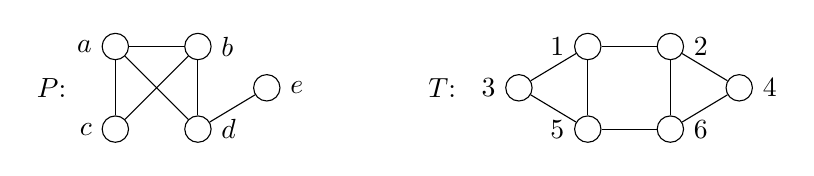
\begin{tikzpicture}
        \node[draw, circle, inner sep=0.5pt] (Na) at (0, 0) {\phantom{0}};
        \node[draw, circle, inner sep=0.5pt, right=0.7 of Na] (Nb) {\phantom{0}};
        \node[draw, circle, inner sep=0.5pt, below=0.7 of Na] (Nc) {\phantom{0}};
        \node[draw, circle, inner sep=0.5pt, right=0.7 of Nc] (Nd) {\phantom{0}};
        \node[draw, circle, inner sep=0.5pt, right=0.7 of $(Nb)!0.5!(Nd)$] (Ne) {\phantom{0}};
        \node[left=0 of Na] {$a$};
        \node[right=0 of Nb] {$b$};
        \node[left=0 of Nc] {$c$};
        \node[right=0 of Nd] {$d$};
        \node[right=0 of Ne] {$e$};
        \node[anchor=east, left=0.5 of $(Na)!0.5!(Nc)$] { $P$: };
        \draw (Na) -- (Nb);
        \draw (Na) -- (Nc);
        \draw (Na) -- (Nd);
        \draw (Nb) -- (Nc);
        \draw (Nb) -- (Nd);
        \draw (Nd) -- (Ne);

        \node[draw, circle, inner sep=0.5pt] (N1) at (6, 0) {\phantom{0}};
        \node[draw, circle, inner sep=0.5pt, right=0.7 of N1] (N2) {\phantom{0}};
        \node[draw, circle, inner sep=0.5pt, below=0.7 of N1] (N5) {\phantom{0}};
        \node[draw, circle, inner sep=0.5pt, below=0.7 of N2] (N6) {\phantom{0}};
        \node[draw, circle, inner sep=0.5pt, right=0.7 of $(N2)!0.5!(N6)$] (N4) {\phantom{0}};
        \node[draw, circle, inner sep=0.5pt, left=0.7 of $(N1)!0.5!(N5)$] (N3) {\phantom{0}};
        \node[left=0 of N1] {$1$};
        \node[right=0 of N2] {$2$};
        \node[left=0 of N3] {$3$};
        \node[right=0 of N4] {$4$};
        \node[left=0 of N5] {$5$};
        \node[right=0 of N6] {$6$};
        \node[anchor=east, left=0.5 of N3] { $T$: };
        \draw (N1) -- (N2);
        \draw (N1) -- (N3);
        \draw (N1) -- (N5);
        \draw (N2) -- (N4);
        \draw (N2) -- (N6);
        \draw (N3) -- (N5);
        \draw (N4) -- (N6);
        \draw (N5) -- (N6);
    \end{tikzpicture}

    \bigskip

    \bigskip

    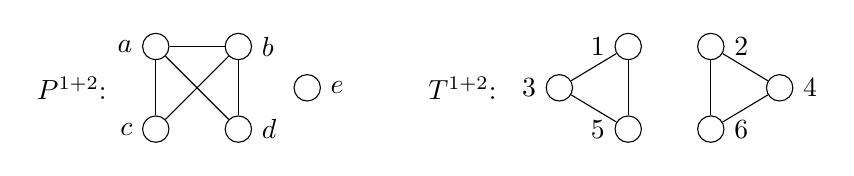
\begin{tikzpicture}
        \node[draw, circle, inner sep=0.5pt] (Ma) at (0, -2) {\phantom{0}};
        \node[draw, circle, inner sep=0.5pt, right=0.7 of Ma] (Mb) {\phantom{0}};
        \node[draw, circle, inner sep=0.5pt, below=0.7 of Ma] (Mc) {\phantom{0}};
        \node[draw, circle, inner sep=0.5pt, right=0.7 of Mc] (Md) {\phantom{0}};
        \node[draw, circle, inner sep=0.5pt, right=0.7 of $(Mb)!0.5!(Md)$] (Me) {\phantom{0}};
        \node[left=0 of Ma] {$a$};
        \node[right=0 of Mb] {$b$};
        \node[left=0 of Mc] {$c$};
        \node[right=0 of Md] {$d$};
        \node[right=0 of Me] {$e$};
        \node[anchor=east, left=0.5 of $(Ma)!0.5!(Mc)$] { $P^{1{+}2}$: };
        \draw (Ma) -- (Mb);
        \draw (Ma) -- (Mc);
        \draw (Ma) -- (Md);
        \draw (Mb) -- (Mc);
        \draw (Mb) -- (Md);

        \node[draw, circle, inner sep=0.5pt] (M1) at (6, -2) {\phantom{0}};
        \node[draw, circle, inner sep=0.5pt, right=0.7 of M1] (M2) {\phantom{0}};
        \node[draw, circle, inner sep=0.5pt, below=0.7 of M1] (M5) {\phantom{0}};
        \node[draw, circle, inner sep=0.5pt, below=0.7 of M2] (M6) {\phantom{0}};
        \node[draw, circle, inner sep=0.5pt, right=0.7 of $(M2)!0.5!(M6)$] (M4) {\phantom{0}};
        \node[draw, circle, inner sep=0.5pt, left=0.7 of $(M1)!0.5!(M5)$] (M3) {\phantom{0}};
        \node[left=0 of M1] {$1$};
        \node[right=0 of M2] {$2$};
        \node[left=0 of M3] {$3$};
        \node[right=0 of M4] {$4$};
        \node[left=0 of M5] {$5$};
        \node[right=0 of M6] {$6$};
        \node[anchor=east, left=0.5 of M3] { $T^{1{+}2}$: };
        \draw (M1) -- (M3);
        \draw (M1) -- (M5);
        \draw (M2) -- (M4);
        \draw (M2) -- (M6);
        \draw (M3) -- (M5);
        \draw (M4) -- (M6);
    \end{tikzpicture}\end{center}
\end{frame}

\begin{frame}{Induced Subisomorphisms}
    \begin{itemize}
        \item Find something that is a non-induced subisomorphism \[
                P \rightarrowtail T
            \] and simultaneously a non-induced subisomorphism \[
                \overline{P} \rightarrowtail \overline{T}
            \]
    \end{itemize}
\end{frame}

\begin{frame}{Partially Defined Graphs}
    \begin{itemize}
        \item Challenge for you!
    \end{itemize}
\end{frame}

\begin{frame}{Clique Neighbourhood Filtering}
    \begin{itemize}
        \item If a pattern vertex is contained in a $k$-vertex clique, it must be mapped to a
            target vertex contained in at least a $k$-vertex clique.
        \item Valid without injectivity (with a caveat for loops).
    \end{itemize}

    \bigskip\centering
    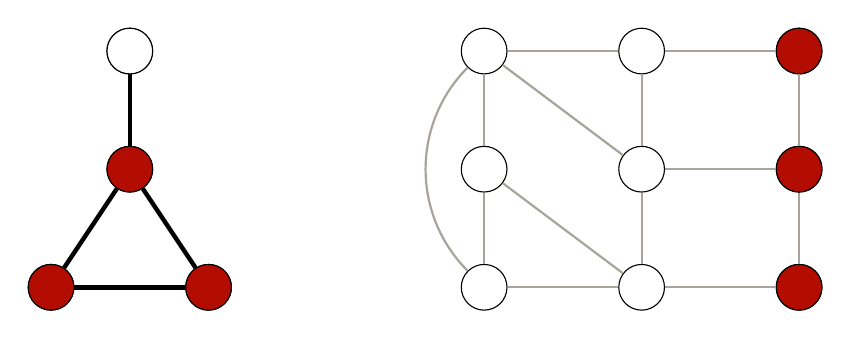
\begin{tikzpicture}
        \node <1> [draw, circle, fill=white, inner sep=4pt, font=\bfseries] (Na) at (1,  0) {\vphantom{1}};
        \node <1> [draw, circle, fill=white, inner sep=4pt, font=\bfseries] (Nb) at (1, -1.5) {\vphantom{1}};
        \node <1> [draw, circle, fill=white, inner sep=4pt, font=\bfseries] (Nc) at (0, -3) {\vphantom{1}};
        \node <1> [draw, circle, fill=white, inner sep=4pt, font=\bfseries] (Nd) at (2, -3) {\vphantom{1}};

        \node <2> [draw, circle, fill=white, inner sep=4pt, font=\bfseries] (Na) at (1,  0) {\vphantom{1}};
        \node <2> [draw, circle, fill=uofgpillarbox, inner sep=4pt, font=\bfseries] (Nb) at (1, -1.5) {\vphantom{1}};
        \node <2> [draw, circle, fill=uofgpillarbox, inner sep=4pt, font=\bfseries] (Nc) at (0, -3) {\vphantom{1}};
        \node <2> [draw, circle, fill=uofgpillarbox, inner sep=4pt, font=\bfseries] (Nd) at (2, -3) {\vphantom{1}};

        \draw [ultra thick] (Na) -- (Nb);
        \draw [ultra thick] (Nb) -- (Nc);
        \draw [ultra thick] (Nc) -- (Nd);
        \draw [ultra thick] (Nb) -- (Nd);

        \node [draw, circle, fill=white, inner sep=4pt, font=\bfseries] (N1) at (5.5,  0) {\vphantom{1}};
        \node [draw, circle, fill=white, inner sep=4pt, font=\bfseries] (N2) at (7.5,  0) {\vphantom{1}};
        \node [draw, circle, fill=white, inner sep=4pt, font=\bfseries] (N3) at (5.5, -1.5) {\vphantom{1}};
        \node [draw, circle, fill=white, inner sep=4pt, font=\bfseries] (N4) at (7.5, -1.5) {\vphantom{1}};
        \node [draw, circle, fill=white, inner sep=4pt, font=\bfseries] (N5) at (5.5, -3) {\vphantom{1}};
        \node [draw, circle, fill=white, inner sep=4pt, font=\bfseries] (N6) at (7.5, -3) {\vphantom{1}};

        \node <1> [draw, circle, fill=white, inner sep=4pt, font=\bfseries] (N7) at (9.5, -3) {\vphantom{1}};
        \node <2> [draw, circle, fill=uofgpillarbox, inner sep=4pt, font=\bfseries] (N7) at (9.5, -3) {\vphantom{1}};
        \node <1> [draw, circle, fill=white, inner sep=4pt, font=\bfseries] (N8) at (9.5, -1.5) {\vphantom{1}};
        \node <2> [draw, circle, fill=uofgpillarbox, inner sep=4pt, font=\bfseries] (N8) at (9.5, -1.5) {\vphantom{1}};
        \node <1> [draw, circle, fill=white, inner sep=4pt, font=\bfseries] (N9) at (9.5, 0) {\vphantom{1}};
        \node <2> [draw, circle, fill=uofgpillarbox, inner sep=4pt, font=\bfseries] (N9) at (9.5, 0) {\vphantom{1}};

        \draw [thick, color=uofgsandstone!50] (N1) -- (N2);
        \draw [thick, color=uofgsandstone!50] (N1) -- (N3);
        \draw [thick, color=uofgsandstone!50] (N1) -- (N4);
        \draw [thick, color=uofgsandstone!50] (N2) -- (N4);
        \draw [thick, color=uofgsandstone!50] (N3) -- (N5);
        \draw [thick, color=uofgsandstone!50] (N3) -- (N6);
        \draw [thick, color=uofgsandstone!50] (N4) -- (N6);
        \draw [thick, color=uofgsandstone!50] (N5) -- (N6);
        \draw [thick, color=uofgsandstone!50] (N1) to [in=135, out=225] (N5);

        \draw [thick, color=uofgsandstone!50] (N7) -- (N8);
        \draw [thick, color=uofgsandstone!50] (N8) -- (N9);
        \draw [thick, color=uofgsandstone!50] (N2) -- (N9);
        \draw [thick, color=uofgsandstone!50] (N4) -- (N8);
        \draw [thick, color=uofgsandstone!50] (N6) -- (N7);
    \end{tikzpicture}
\end{frame}

\section{Search}

\begin{frame}{Variable and Value Ordering Heuristics}
    \begin{itemize}
        \item Variable ordering (i.e.\ pattern vertices): smallest domain first, tie-breaking on highest degree.
            \begin{itemize}
                \item Tends to pick vertices adjacent to things we've already picked.
            \end{itemize}
        \item Value ordering (i.e.\ target vertices): highest degree to lowest.
    \end{itemize}
\end{frame}

\begin{frame}{Sanity Check}
    \begin{center}
        \includegraphics<1>{gen-graph-value-ordering.pdf}
        \includegraphics<2>{gen-graph-value-ordering-unsat.pdf}
    \end{center}
\end{frame}

\section{Detour: Hard Instances}

\begin{frame}[t]{Clique in Random Graphs}
    \begin{center}
        \includegraphics<1>{gen-graph-clique-phase-transition.pdf}
    \end{center}
\end{frame}

\begin{frame}{Let's Generate Random Instances a Different Way}
    \begin{itemize}
        \item Decide upon a pattern graph order (number of vertices) and density.
        \item Decide upon a target graph order and density.
        \item Generate instances at random, independently.
    \end{itemize}
\end{frame}

\begin{frame}{When is Non-Induced Subgraph Isomorphism Hard?}
    \begin{center}
        \only<1>{
            \includegraphics<1>{gen-graph-phase-transition.pdf}
        }\only<2>{
            \begin{tikzpicture}[every node/.style={inner sep=0pt, outer sep=0pt, column sep=10pt}, ampersand replacement=\&]
                \matrix {
                    \node [anchor=center] {}; \&
                \node [anchor=center] {\tiny $G(10, x) \rightarrowtail G(150, y)$}; \&
                \node [anchor=center] {\tiny $G(20, x) \rightarrowtail G(150, y)$}; \&
                \node [anchor=center] {\tiny $G(30, x) \rightarrowtail G(150, y)$}; \&
                \\[0.1cm]
                \node [anchor=center, inner sep=2pt] [rotate=90] {\tiny Satisfiable?}; \&
                \node [anchor=center] {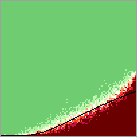
\includegraphics{gen-graph-non-induced-satisfiable-10-150.pdf}}; \&
                \node [anchor=center] {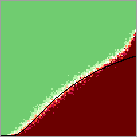
\includegraphics{gen-graph-non-induced-satisfiable-20-150.pdf}}; \&
                \node [anchor=center] {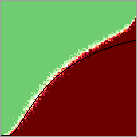
\includegraphics{gen-graph-non-induced-satisfiable-30-150.pdf}}; \&
                \\[0.2cm]
                \node [anchor=center, inner sep=2pt] [rotate=90] {\tiny Glasgow Nodes}; \&
                \node [anchor=center] {
\includegraphics{gen-graph-non-induced-nodes-10-150.pdf}}; \&
                \node [anchor=center] {
\includegraphics{gen-graph-non-induced-nodes-20-150.pdf}}; \&
                \node [anchor=center] {
\includegraphics{gen-graph-non-induced-nodes-30-150.pdf}}; \&
                \\
            };
            \end{tikzpicture}
        }\only<3>{
            \begin{tikzpicture}[every node/.style={inner sep=0pt, outer sep=0pt, column sep=10pt}, ampersand replacement=\&]
                \matrix {
                    \node [anchor=center] {}; \&
                \node [anchor=center] {\tiny $G(10, x) \rightarrowtail G(150, y)$}; \&
                \node [anchor=center] {\tiny $G(20, x) \rightarrowtail G(150, y)$}; \&
                \node [anchor=center] {\tiny $G(30, x) \rightarrowtail G(150, y)$}; \&
                \\[0.1cm]
                \node [anchor=center, inner sep=2pt] [rotate=90] {\tiny Satisfiable?}; \&
                \node [anchor=center] {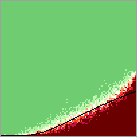
\includegraphics{gen-graph-non-induced-satisfiable-10-150.pdf}}; \&
                \node [anchor=center] {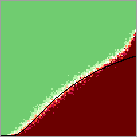
\includegraphics{gen-graph-non-induced-satisfiable-20-150.pdf}}; \&
                \node [anchor=center] {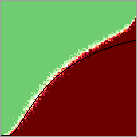
\includegraphics{gen-graph-non-induced-satisfiable-30-150.pdf}}; \&
                \\[0.2cm]
                \node [anchor=center, inner sep=2pt] [rotate=90] {\tiny LAD Nodes}; \&
                \node [anchor=center] {
\includegraphics{gen-graph-lad-non-induced-nodes-10-150.pdf}}; \&
                \node [anchor=center] {
\includegraphics{gen-graph-lad-non-induced-nodes-20-150.pdf}}; \&
                \node [anchor=center] {
\includegraphics{gen-graph-lad-non-induced-nodes-30-150.pdf}}; \&
                \\
            };
            \end{tikzpicture}
        }\only<4>{
            \begin{tikzpicture}[every node/.style={inner sep=0pt, outer sep=0pt, column sep=10pt}, ampersand replacement=\&]
                \matrix {
                    \node [anchor=center] {}; \&
                \node [anchor=center] {\tiny $G(10, x) \rightarrowtail G(150, y)$}; \&
                \node [anchor=center] {\tiny $G(20, x) \rightarrowtail G(150, y)$}; \&
                \node [anchor=center] {\tiny $G(30, x) \rightarrowtail G(150, y)$}; \&
                \\[0.1cm]
                \node [anchor=center, inner sep=2pt] [rotate=90] {\tiny Satisfiable?}; \&
                \node [anchor=center] {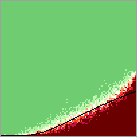
\includegraphics{gen-graph-non-induced-satisfiable-10-150.pdf}}; \&
                \node [anchor=center] {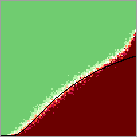
\includegraphics{gen-graph-non-induced-satisfiable-20-150.pdf}}; \&
                \node [anchor=center] {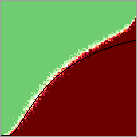
\includegraphics{gen-graph-non-induced-satisfiable-30-150.pdf}}; \&
                \\[0.2cm]
                \node [anchor=center, inner sep=2pt] [rotate=90] {\tiny VF2 Nodes}; \&
                \node [anchor=center] {
\includegraphics{gen-graph-vf2-non-induced-nodes-10-150.pdf}}; \&
                \node [anchor=center] {
\includegraphics{gen-graph-vf2-non-induced-nodes-20-150.pdf}}; \&
                \node [anchor=center] {
\includegraphics{gen-graph-vf2-non-induced-nodes-30-150.pdf}}; \&
                \\
            };
            \end{tikzpicture}
        }
    \end{center}
\end{frame}

\begin{frame}{Hand-Wavy Theoretical Justification}
    \begin{itemize}
        \item Maximise the expected number of solutions during search?
        \item If $P = G(p, q)$ and $T = G(t, u)$,
            \begin{equation*} \langle Sol \rangle = \underbrace{t \cdot (t - 1) \cdot \ldots \cdot (t
                - p + 1)}_{\textnormal{injective mapping}} \cdot \underbrace{\vphantom{(p)}{u}^{q \cdot
            \binom{p}{2}}}_{\textnormal{adjacency}} \end{equation*}
        \item Smallest domain first keeps remaining domain sizes large.
        \item High pattern degree makes the remaining pattern subgraph sparser, reducing $q$.
        \item High target degree leaves as many vertices as possible available for future
            use, making $u$ larger.
    \end{itemize}
\end{frame}

\begin{frame}{Induced is Much More Complicated}
    \begin{center}
        \only<1>{
    \begin{tikzpicture}[every node/.style={inner sep=0pt, outer sep=0pt, column sep=6pt}, ampersand replacement=\&]
        \matrix {
                    \node [anchor=center] {}; \&
            \node [anchor=center] {\tiny $G(10, x) \hookrightarrow G(150, y)$}; \&
            \node [anchor=center] {\tiny $G(14, x) \hookrightarrow G(150, y)$}; \&
            \node [anchor=center] {\tiny $G(16, x) \hookrightarrow G(150, y)$}; \&
            \node [anchor=center] {\tiny $G(20, x) \hookrightarrow G(150, y)$}; \&
            \\[0.1cm]
                \node [anchor=center, inner sep=2pt] [rotate=90] {\tiny Satisfiable?}; \&
            \node [anchor=center] {
\includegraphics{gen-graph-induced-satisfiable-10-150.pdf}}; \&
            \node [anchor=center] {
\includegraphics{gen-graph-induced-satisfiable-14-150.pdf}}; \&
            \node [anchor=center] {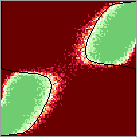
\includegraphics{gen-graph-induced-satisfiable-16-150.pdf}}; \&
            \node [anchor=center] {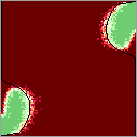
\includegraphics{gen-graph-induced-satisfiable-20-150.pdf}}; \&
            \\[0.2cm]
                \node [anchor=center, inner sep=2pt] [rotate=90] {\tiny Glasgow Nodes}; \&
            \node [anchor=center] {
\includegraphics{gen-graph-induced-nodes-10-150.pdf}}; \&
            \node [anchor=center] {
\includegraphics{gen-graph-induced-nodes-14-150.pdf}}; \&
            \node [anchor=center] {
\includegraphics{gen-graph-induced-nodes-16-150.pdf}}; \&
            \node [anchor=center] {
\includegraphics{gen-graph-induced-nodes-20-150.pdf}}; \&
            \\
        };
    \end{tikzpicture}
}\only<2>{
    \begin{tikzpicture}[every node/.style={inner sep=0pt, outer sep=0pt, column sep=6pt}, ampersand replacement=\&]
        \matrix {
                    \node [anchor=center] {}; \&
            \node [anchor=center] {\tiny $G(10, x) \hookrightarrow G(150, y)$}; \&
            \node [anchor=center] {\tiny $G(14, x) \hookrightarrow G(150, y)$}; \&
            \node [anchor=center] {\tiny $G(16, x) \hookrightarrow G(150, y)$}; \&
            \node [anchor=center] {\tiny $G(20, x) \hookrightarrow G(150, y)$}; \&
            \\[0.1cm]
                \node [anchor=center, inner sep=2pt] [rotate=90] {\tiny Satisfiable?}; \&
            \node [anchor=center] {
\includegraphics{gen-graph-induced-satisfiable-10-150.pdf}}; \&
            \node [anchor=center] {
\includegraphics{gen-graph-induced-satisfiable-14-150.pdf}}; \&
            \node [anchor=center] {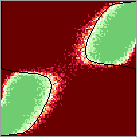
\includegraphics{gen-graph-induced-satisfiable-16-150.pdf}}; \&
            \node [anchor=center] {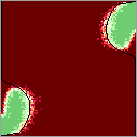
\includegraphics{gen-graph-induced-satisfiable-20-150.pdf}}; \&
            \\[0.2cm]
                \node [anchor=center, inner sep=2pt] [rotate=90] {\tiny LAD Nodes}; \&
            \node [anchor=center] {
\includegraphics{gen-graph-lad-induced-nodes-10-150.pdf}}; \&
            \node [anchor=center] {
\includegraphics{gen-graph-lad-induced-nodes-14-150.pdf}}; \&
            \node [anchor=center] {
\includegraphics{gen-graph-lad-induced-nodes-16-150.pdf}}; \&
            \node [anchor=center] {
\includegraphics{gen-graph-lad-induced-nodes-20-150.pdf}}; \&
            \\
        };
    \end{tikzpicture}
}\only<3>{
    \begin{tikzpicture}[every node/.style={inner sep=0pt, outer sep=0pt, column sep=6pt}, ampersand replacement=\&]
        \matrix {
                    \node [anchor=center] {}; \&
            \node [anchor=center] {\tiny $G(10, x) \hookrightarrow G(150, y)$}; \&
            \node [anchor=center] {\tiny $G(14, x) \hookrightarrow G(150, y)$}; \&
            \node [anchor=center] {\tiny $G(16, x) \hookrightarrow G(150, y)$}; \&
            \node [anchor=center] {\tiny $G(20, x) \hookrightarrow G(150, y)$}; \&
            \\[0.1cm]
                \node [anchor=center, inner sep=2pt] [rotate=90] {\tiny Satisfiable?}; \&
            \node [anchor=center] {
\includegraphics{gen-graph-induced-satisfiable-10-150.pdf}}; \&
            \node [anchor=center] {
\includegraphics{gen-graph-induced-satisfiable-14-150.pdf}}; \&
            \node [anchor=center] {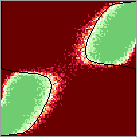
\includegraphics{gen-graph-induced-satisfiable-16-150.pdf}}; \&
            \node [anchor=center] {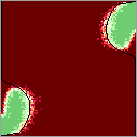
\includegraphics{gen-graph-induced-satisfiable-20-150.pdf}}; \&
            \\[0.2cm]
                \node [anchor=center, inner sep=2pt] [rotate=90] {\tiny VF2 Nodes}; \&
            \node [anchor=center] {
\includegraphics{gen-graph-vf2-induced-nodes-10-150.pdf}}; \&
            \node [anchor=center] {
\includegraphics{gen-graph-vf2-induced-nodes-14-150.pdf}}; \&
            \node [anchor=center] {
\includegraphics{gen-graph-vf2-induced-nodes-16-150.pdf}}; \&
            \node [anchor=center] {
\includegraphics{gen-graph-vf2-induced-nodes-20-150.pdf}}; \&
            \\
        };
    \end{tikzpicture}
}\only<4>{
    \begin{tikzpicture}[every node/.style={inner sep=0pt, outer sep=0pt, column sep=6pt}, ampersand replacement=\&]
        \matrix {
                    \node [anchor=center] {}; \&
            \node [anchor=center] {\tiny $G(10, x) \hookrightarrow G(150, y)$}; \&
            \node [anchor=center] {\tiny $G(14, x) \hookrightarrow G(150, y)$}; \&
            \node [anchor=center] {\tiny $G(16, x) \hookrightarrow G(150, y)$}; \&
            \node [anchor=center] {\tiny $G(20, x) \hookrightarrow G(150, y)$}; \&
            \\[0.1cm]
                \node [anchor=center, inner sep=2pt] [rotate=90] {\tiny Satisfiable?}; \&
            \node [anchor=center] {
\includegraphics{gen-graph-induced-satisfiable-10-150.pdf}}; \&
            \node [anchor=center] {
\includegraphics{gen-graph-induced-satisfiable-14-150.pdf}}; \&
            \node [anchor=center] {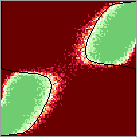
\includegraphics{gen-graph-induced-satisfiable-16-150.pdf}}; \&
            \node [anchor=center] {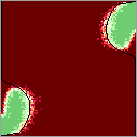
\includegraphics{gen-graph-induced-satisfiable-20-150.pdf}}; \&
            \\[0.2cm] \node [anchor=center, inner sep=2pt] [rotate=90] {\tiny VF3 Nodes}; \&
            \node [anchor=center] {\includegraphics{gen-graph-vf3-induced-nodes-10-150.pdf}}; \&
            \node [anchor=center] {\includegraphics{gen-graph-vf3-induced-nodes-14-150.pdf}}; \&
            \node [anchor=center] {\includegraphics{gen-graph-vf3-induced-nodes-16-150.pdf}}; \&
            \node [anchor=center] {\includegraphics{gen-graph-vf3-induced-nodes-20-150.pdf}}; \&
            \\
        };
    \end{tikzpicture}
}
    \end{center}
\end{frame}

\begin{frame}{Is This Algorithm-Independent?}
    \begin{center}
        \only<1>{
    \begin{tikzpicture}[every node/.style={inner sep=0pt, outer sep=0pt, column sep=6pt}, ampersand replacement=\&]
        \matrix {
            \node [anchor=center] {}; \&
            \node [anchor=center] {\tiny $G(10, x) \hookrightarrow G(75, y)$}; \&
            \node [anchor=center] {\tiny $G(14, x) \hookrightarrow G(75, y)$}; \&
            \node [anchor=center] {\tiny $G(16, x) \hookrightarrow G(75, y)$}; \&
            \node [anchor=center] {\tiny $G(18, x) \hookrightarrow G(75, y)$}; \&
            \\[0.1cm]
            \node [anchor=center, inner sep=2pt] [rotate=90] {\tiny Satisfiable?}; \&
            \node [anchor=center] {\includegraphics{gen-graph-induced-satisfiable-10-75.pdf}}; \&
            \node [anchor=center] {\includegraphics{gen-graph-induced-satisfiable-14-75.pdf}}; \&
            \node [anchor=center] {\includegraphics{gen-graph-induced-satisfiable-16-75.pdf}}; \&
            \node [anchor=center] {\includegraphics{gen-graph-induced-satisfiable-18-75.pdf}}; \&
            \\[0.2cm] \node [anchor=center, inner sep=2pt] [rotate=90] {\tiny Glucose (SAT)}; \&
            \node [anchor=center] {\includegraphics{gen-graph-glucose-induced-nodes-10-75.pdf}}; \&
            \node [anchor=center] {\includegraphics{gen-graph-glucose-induced-nodes-14-75.pdf}}; \&
            \node [anchor=center] {\includegraphics{gen-graph-glucose-induced-nodes-16-75.pdf}}; \&
            \node [anchor=center] {\includegraphics{gen-graph-glucose-induced-nodes-18-75.pdf}}; \&
            \\
        };
    \end{tikzpicture}}\only<2>{
    \begin{tikzpicture}[every node/.style={inner sep=0pt, outer sep=0pt, column sep=6pt}, ampersand replacement=\&]
        \matrix {
            \node [anchor=center] {}; \&
            \node [anchor=center] {\tiny $G(10, x) \hookrightarrow G(75, y)$}; \&
            \node [anchor=center] {\tiny $G(14, x) \hookrightarrow G(75, y)$}; \&
            \node [anchor=center] {\tiny $G(16, x) \hookrightarrow G(75, y)$}; \&
            \node [anchor=center] {\tiny $G(18, x) \hookrightarrow G(75, y)$}; \&
            \\[0.1cm]
            \node [anchor=center, inner sep=2pt] [rotate=90] {\tiny Satisfiable?}; \&
            \node [anchor=center] {\includegraphics{gen-graph-induced-satisfiable-10-75.pdf}}; \&
            \node [anchor=center] {\includegraphics{gen-graph-induced-satisfiable-14-75.pdf}}; \&
            \node [anchor=center] {\includegraphics{gen-graph-induced-satisfiable-16-75.pdf}}; \&
            \node [anchor=center] {\includegraphics{gen-graph-induced-satisfiable-18-75.pdf}}; \&
            \\[0.2cm] \node [anchor=center, inner sep=2pt] [rotate=90] {\tiny Clasp (PB)}; \&
            \node [anchor=center] {\includegraphics{gen-graph-clasp-induced-nodes-10-75.pdf}}; \&
            \node [anchor=center] {\includegraphics{gen-graph-clasp-induced-nodes-14-75.pdf}}; \&
            \node [anchor=center] {\includegraphics{gen-graph-clasp-induced-nodes-16-75.pdf}}; \&
            \node [anchor=center] {\includegraphics{gen-graph-clasp-induced-nodes-18-75.pdf}}; \&
            \\
        };
    \end{tikzpicture}}\only<3>{
    \begin{tikzpicture}[every node/.style={inner sep=0pt, outer sep=0pt, column sep=6pt}, ampersand replacement=\&]
        \matrix {
            \node [anchor=center] {}; \&
            \node [anchor=center] {\tiny $G(10, x) \hookrightarrow G(75, y)$}; \&
            \node [anchor=center] {\tiny $G(14, x) \hookrightarrow G(75, y)$}; \&
            \node [anchor=center] {\tiny $G(16, x) \hookrightarrow G(75, y)$}; \&
            \node [anchor=center] {\tiny $G(18, x) \hookrightarrow G(75, y)$}; \&
            \\[0.1cm]
            \node [anchor=center, inner sep=2pt] [rotate=90] {\tiny Satisfiable?}; \&
            \node [anchor=center] {\includegraphics{gen-graph-induced-satisfiable-10-75.pdf}}; \&
            \node [anchor=center] {\includegraphics{gen-graph-induced-satisfiable-14-75.pdf}}; \&
            \node [anchor=center] {\includegraphics{gen-graph-induced-satisfiable-16-75.pdf}}; \&
            \node [anchor=center] {\includegraphics{gen-graph-induced-satisfiable-18-75.pdf}}; \&
            \\[0.2cm] \node [anchor=center, inner sep=2pt] [rotate=90] {\tiny BBMC (Clique)}; \&
            \node [anchor=center] {\includegraphics{gen-graph-clique-induced-nodes-10-75.pdf}}; \&
            \node [anchor=center] {\includegraphics{gen-graph-clique-induced-nodes-14-75.pdf}}; \&
            \node [anchor=center] {\includegraphics{gen-graph-clique-induced-nodes-16-75.pdf}}; \&
            \node [anchor=center] {\includegraphics{gen-graph-clique-induced-nodes-18-75.pdf}}; \&
            \\
        };
    \end{tikzpicture}}\only<4>{
    \begin{tikzpicture}[every node/.style={inner sep=0pt, outer sep=0pt, column sep=6pt}, ampersand replacement=\&]
        \matrix {
            \node [anchor=center] {}; \&
            \node [anchor=center] {\tiny $G(10, x) \hookrightarrow G(75, y)$}; \&
            \node [anchor=center] {\tiny $G(14, x) \hookrightarrow G(75, y)$}; \&
            \node [anchor=center] {\tiny $G(16, x) \hookrightarrow G(75, y)$}; \&
            \node [anchor=center] {\tiny $G(18, x) \hookrightarrow G(75, y)$}; \&
            \\[0.1cm]
            \node [anchor=center, inner sep=2pt] [rotate=90] {\tiny Satisfiable?}; \&
            \node [anchor=center] {\includegraphics{gen-graph-induced-satisfiable-10-75.pdf}}; \&
            \node [anchor=center] {\includegraphics{gen-graph-induced-satisfiable-14-75.pdf}}; \&
            \node [anchor=center] {\includegraphics{gen-graph-induced-satisfiable-16-75.pdf}}; \&
            \node [anchor=center] {\includegraphics{gen-graph-induced-satisfiable-18-75.pdf}}; \&
            \\[0.2cm] \node [anchor=center, inner sep=2pt] [rotate=90] {\tiny Gurobi (MIP)}; \&
            \node [anchor=center] {\includegraphics{gen-graph-gurobi-induced-nodes-10-75.pdf}}; \&
            \node [anchor=center] {\includegraphics{gen-graph-gurobi-induced-nodes-14-75.pdf}}; \&
            \node [anchor=center] {\includegraphics{gen-graph-gurobi-induced-nodes-16-75.pdf}}; \&
            \node [anchor=center] {\includegraphics{gen-graph-gurobi-induced-nodes-18-75.pdf}}; \&
            \\
        };
    \end{tikzpicture}}
    \end{center}
\end{frame}

\begin{frame}{Constrainedness}
    \only<1>{\begin{equation*}\label{equation:constrainedness}\kappa = 1 - \frac{\log \left( t^{\underline{p}}
\cdot {u}^{q \cdot \binom{p}{2}} \cdot {(1 - u)}^{(1 - q) \cdot \binom{p}{2}}
    \right)}{\log t^{\underline{p}}} \end{equation*}}\only<2>{
    \centering\begin{tikzpicture}[every node/.style={inner sep=0pt, outer sep=0pt, column sep=6pt}, ampersand replacement=\&]
        \matrix {
                    \node [anchor=center] {}; \&
            \node [anchor=center] {\tiny $G(10, x) \hookrightarrow G(150, y)$}; \&
            \node [anchor=center] {\tiny $G(14, x) \hookrightarrow G(150, y)$}; \&
            \node [anchor=center] {\tiny $G(16, x) \hookrightarrow G(150, y)$}; \&
            \node [anchor=center] {\tiny $G(20, x) \hookrightarrow G(150, y)$}; \&
            \\[0.1cm]
                \node [anchor=center, inner sep=2pt] [rotate=90] {\tiny Satisfiable?}; \&
            \node [anchor=center] {\includegraphics{gen-graph-induced-kappa-10-150.pdf}}; \&
            \node [anchor=center] {\includegraphics{gen-graph-induced-kappa-14-150.pdf}}; \&
            \node [anchor=center] {\includegraphics{gen-graph-induced-kappa-16-150.pdf}}; \&
            \node [anchor=center] {\includegraphics{gen-graph-induced-kappa-20-150.pdf}}; \&
            \\[0.2cm] \node [anchor=center, inner sep=2pt] [rotate=90] {\tiny Glasgow Nodes}; \&
            \node [anchor=center] {\includegraphics{gen-graph-induced-nodes-10-150.pdf}}; \&
            \node [anchor=center] {\includegraphics{gen-graph-induced-nodes-14-150.pdf}}; \&
            \node [anchor=center] {\includegraphics{gen-graph-induced-nodes-16-150.pdf}}; \&
            \node [anchor=center] {\includegraphics{gen-graph-induced-nodes-20-150.pdf}}; \&
            \\
        };
    \end{tikzpicture}
    }
\end{frame}

\begin{frame}{Labelled Subgraph Isomorphism}
    \begin{itemize}
        \item Vertices have labels, and the isomorphism must preserve labels.
        \item Carbon must map to carbon, hydrogen to hydrogen, \ldots
    \end{itemize}

    \begin{equation*}\label{equation:non-induced-labelled-prediction} \langle Sol \rangle = \left(
        \frac{\Gamma\left(\nicefrac{t}{k} + 1\right)}{\Gamma\left(\nicefrac{t}{k} - \nicefrac{p}{k} +
        1\right)} \right)^{k}  \cdot
    {u}^{q \cdot \binom{p}{2}} \end{equation*}
\end{frame}

\begin{frame}{Labels and Phase Transitions}
    \begin{center}
        \only<1>{
    \begin{tikzpicture}[every node/.style={inner sep=0pt, outer sep=0pt, column sep=6pt}, ampersand replacement=\&]
        \matrix {
                    \node [anchor=center] {}; \&
            \node [anchor=center] {\tiny $G(20, x, 1) \hookrightarrow G(150, y, 1)$}; \&
            \node [anchor=center] {\tiny $G(20, x, 2) \hookrightarrow G(150, y, 2)$}; \&
            \node [anchor=center] {\tiny $G(20, x, 5) \hookrightarrow G(150, y, 5)$}; \&
            \node [anchor=center] {\tiny $G(20, x, 20) \hookrightarrow G(150, y, 20)$}; \&
            \\[0.1cm]
                \node [anchor=center, inner sep=2pt] [rotate=90] {\tiny Satisfiable?}; \&
            \node [anchor=center] {\includegraphics{gen-graph-non-induced-satisfiable-20-150.pdf}}; \&
            \node [anchor=center] {\includegraphics{gen-graph-non-induced-satisfiable-20-l2-150.pdf}}; \&
            \node [anchor=center] {\includegraphics{gen-graph-non-induced-satisfiable-20-l5-150.pdf}}; \&
            \node [anchor=center] {\includegraphics{gen-graph-non-induced-satisfiable-20-l20-150.pdf}}; \&
            \\[0.2cm]
                \node [anchor=center, inner sep=2pt] [rotate=90] {\tiny Glasgow Nodes}; \&
            \node [anchor=center] {\includegraphics{gen-graph-non-induced-nodes-20-150.pdf}}; \&
            \node [anchor=center] {\includegraphics{gen-graph-non-induced-nodes-20-l2-150.pdf}}; \&
            \node [anchor=center] {\includegraphics{gen-graph-non-induced-nodes-20-l5-150.pdf}}; \&
            \node [anchor=center] {\includegraphics{gen-graph-non-induced-nodes-20-l20-150.pdf}}; \&
            \\
        };
    \end{tikzpicture}
}\only<2>{
    \begin{tikzpicture}[every node/.style={inner sep=0pt, outer sep=0pt, column sep=6pt}, ampersand replacement=\&]
        \matrix {
                    \node [anchor=center] {}; \&
            \node [anchor=center] {\tiny $G(20, x, 1) \hookrightarrow G(150, y, 1)$}; \&
            \node [anchor=center] {\tiny $G(20, x, 2) \hookrightarrow G(150, y, 2)$}; \&
            \node [anchor=center] {\tiny $G(20, x, 5) \hookrightarrow G(150, y, 5)$}; \&
            \node [anchor=center] {\tiny $G(20, x, 20) \hookrightarrow G(150, y, 20)$}; \&
            \\[0.1cm]
                \node [anchor=center, inner sep=2pt] [rotate=90] {\tiny Satisfiable?}; \&
            \node [anchor=center] {\includegraphics{gen-graph-non-induced-satisfiable-20-150.pdf}}; \&
            \node [anchor=center] {\includegraphics{gen-graph-non-induced-satisfiable-20-l2-150.pdf}}; \&
            \node [anchor=center] {\includegraphics{gen-graph-non-induced-satisfiable-20-l5-150.pdf}}; \&
            \node [anchor=center] {\includegraphics{gen-graph-non-induced-satisfiable-20-l20-150.pdf}}; \&
            \\[0.2cm]
                \node [anchor=center, inner sep=2pt] [rotate=90] {\tiny LAD Nodes}; \&
            \node [anchor=center] {\includegraphics{gen-graph-lad-non-induced-nodes-20-150.pdf}}; \&
            \node [anchor=center] {\includegraphics{gen-graph-lad-non-induced-nodes-20-l2-150.pdf}}; \&
            \node [anchor=center] {\includegraphics{gen-graph-lad-non-induced-nodes-20-l5-150.pdf}}; \&
            \node [anchor=center] {\includegraphics{gen-graph-lad-non-induced-nodes-20-l20-150.pdf}}; \&
            \\
        };
    \end{tikzpicture}
}\only<3>{
    \begin{tikzpicture}[every node/.style={inner sep=0pt, outer sep=0pt, column sep=6pt}, ampersand replacement=\&]
        \matrix {
                    \node [anchor=center] {}; \&
            \node [anchor=center] {\tiny $G(20, x, 1) \hookrightarrow G(150, y, 1)$}; \&
            \node [anchor=center] {\tiny $G(20, x, 2) \hookrightarrow G(150, y, 2)$}; \&
            \node [anchor=center] {\tiny $G(20, x, 5) \hookrightarrow G(150, y, 5)$}; \&
            \node [anchor=center] {\tiny $G(20, x, 20) \hookrightarrow G(150, y, 20)$}; \&
            \\[0.1cm]
                \node [anchor=center, inner sep=2pt] [rotate=90] {\tiny Satisfiable?}; \&
            \node [anchor=center] {\includegraphics{gen-graph-non-induced-satisfiable-20-150.pdf}}; \&
            \node [anchor=center] {\includegraphics{gen-graph-non-induced-satisfiable-20-l2-150.pdf}}; \&
            \node [anchor=center] {\includegraphics{gen-graph-non-induced-satisfiable-20-l5-150.pdf}}; \&
            \node [anchor=center] {\includegraphics{gen-graph-non-induced-satisfiable-20-l20-150.pdf}}; \&
            \\[0.2cm]
                \node [anchor=center, inner sep=2pt] [rotate=90] {\tiny VF2 Nodes}; \&
            \node [anchor=center] {\includegraphics{gen-graph-vf2-non-induced-nodes-20-150.pdf}}; \&
            \node [anchor=center] {\includegraphics{gen-graph-vf2-non-induced-nodes-20-l2-150.pdf}}; \&
            \node [anchor=center] {\includegraphics{gen-graph-vf2-non-induced-nodes-20-l5-150.pdf}}; \&
            \node [anchor=center] {\includegraphics{gen-graph-vf2-non-induced-nodes-20-l20-150.pdf}}; \&
            \\
        };
    \end{tikzpicture}
}
    \end{center}
\end{frame}

\begin{frame}{Connectivity Algorithms are Really Stupid}
    \centering
    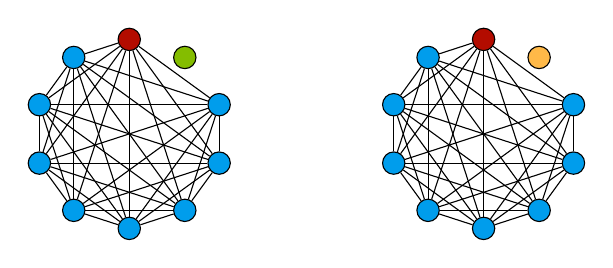
\begin{tikzpicture}[scale=0.5,every node/.style={font=\footnotesize}]
        \begin{scope}
            \newcount \myc
            \newcount \myd
            \newcount \mye
            \foreach \n in {1, ..., 8}{
                \myc=\n \advance\myc by -1 \multiply\myc by -360 \divide\myc by 10 \advance\myc by 18
                \node[draw, circle, fill=uofgcobalt, inner sep=0.5pt] (N\n) at (\the\myc:2.4) {\phantom{0}};
            }
            \node[draw, circle, fill=uofgpillarbox, inner sep=0.5pt] (N9) at (90.0:2.4) {\phantom{0}};
            \node[draw, circle, fill=uofglawn, inner sep=0.5pt] (N10) at (54.0:2.4) {\phantom{0}};

            \foreach \n in {1, ..., 8}{
                \myd=\n
                \myc=\n \advance\myc by 1
                \foreach \m in {\the\myc, ..., 9}{
                    \mye=\m
                    \draw (N\the\myd) -- (N\the\mye);
                }
            }
        \end{scope}
        \begin{scope}[xshift=9cm]
            \newcount \myc
            \newcount \myd
            \newcount \mye
            \foreach \n in {1, ..., 8}{
                \myc=\n \advance\myc by -1 \multiply\myc by -360 \divide\myc by 10 \advance\myc by 18
                \node[draw, circle, fill=uofgcobalt, inner sep=0.5pt] (N\n) at (\the\myc:2.4) {\phantom{0}};
            }
            \node[draw, circle, fill=uofgpillarbox, inner sep=0.5pt] (N9) at (90.0:2.4) {\phantom{0}};
            \node[draw, circle, fill=uofgpumpkin, inner sep=0.5pt] (N10) at (54.0:2.4) {\phantom{0}};

            \foreach \n in {1, ..., 8}{
                \myd=\n
                \myc=\n \advance\myc by 1
                \foreach \m in {\the\myc, ..., 9}{
                    \mye=\m
                    \draw (N\the\myd) -- (N\the\mye);
                }
            }
        \end{scope}
    \end{tikzpicture}
\end{frame}

\section{Back to Search}

\begin{frame}{Back to Value-Ordering Heuristics}
    \begin{itemize}
        \item Largest target degree first.
    \end{itemize}
\end{frame}

\begin{frame}{However\ldots}
    \begin{itemize}
        \item What if several vertices have the same degree?
        \item Is a vertex of degree $10$ really that much better than a vertex of degree $9$?
    \end{itemize}
\end{frame}

\begin{frame}{Discrepancy Search?}
    \begin{center}
        \includegraphics<1>{gen-graph-value-ordering-dds.pdf}%
        \includegraphics<2>{gen-graph-value-ordering-dds-unsat.pdf}%
        \includegraphics<3>{gen-graph-value-ordering-dds-scatter.pdf}
    \end{center}
\end{frame}

\begin{frame}{Random Search with Restarts and Nogood Recording}
    \only<1>{\begin{itemize}
        \item Back to the random value-ordering heuristic.
        \item Aggressive restarts: every 100ms.
        \item Nogood recording and 2WL to avoid repeating work.
    \end{itemize}}\only<2->{
    \begin{center}
        \includegraphics<2>{gen-graph-rsr.pdf}%
        \includegraphics<3>{gen-graph-rsr-scatter.pdf}%
    \end{center}}
\end{frame}


\begin{frame}{Value-Ordering Heuristics as Distributions}
    \begin{itemize}
        \item Traditional view: value-ordering defines a search order.
        \item New view: value-ordering defines \textcolor{uofgcobalt}{what proportion of the search
            effort} should be spent on different subproblems.
        \item According to people who know more statistics than me, if solutions are uniformly
            distributed, then random search with restarts should be better than DFS.
    \end{itemize}
\end{frame}

\begin{frame}{A Slightly Random Value-Ordering Heuristic}
    \only<1>{
    \begin{itemize}
        \item For a fixed domain $D_v$, pick a vertex $v'$ from a domain $D_v$ with probability
    \[ p(v') = \frac{2^{\deg(v')}}{\sum_{w \in D_v}{2^{\deg(w)}}} \]
        \item Equally likely to pick between two vertices of degree $d$.
        \item Twice as likely to select a vertex of degree $d$ than a vertex of degree $d - 1$.
        \item Justification: \textcolor{uofgcobalt}{solution density} and expected distribution of solutions.
    \end{itemize}}\only<2>{
    \begin{center}
        \includegraphics<2>{gen-graph-bias-scatter.pdf}%
    \end{center}}
\end{frame}

\begin{frame}{Is It Better?}
    \begin{center}
        \includegraphics<1>{gen-graph-sbs-scatter.pdf}%
        \includegraphics<2>{gen-graph-sbs.pdf}%
    \end{center}
\end{frame}

\begin{frame}{Parallel Search}
    \begin{itemize}
        \item Each thread gets its own random seed.
        \item Barrier synchronise on restarts.
        \item Share nogoods.
    \end{itemize}
\end{frame}

\begin{frame}{Is It Even Betterer?}
    \begin{center}
    \includegraphics<1>{gen-graph-par-scatter.pdf}%
    \includegraphics<2>{gen-graph-par.pdf}%
    \includegraphics<3>{gen-graph-dist.pdf}%
    \end{center}
\end{frame}

\section{Summary}

\begin{frame}{Lessons Learned}
    \begin{itemize}
        \item Got to get a lot of things right:
            \begin{itemize}
                \item Design.
                \item Engineering.
                \item Evaluation.
                \item Understanding the hardware.
            \end{itemize}
        \item Being clever only pays off if you can do it quickly.
            \begin{itemize}
                \item Except sometimes it pays off even if it's really expensive.
            \end{itemize}
        \item Not always clear what problem people really want to solve.
    \end{itemize}
\end{frame}

\section{Research Topics}

\begin{frame}{Symmetries}
    \centering
    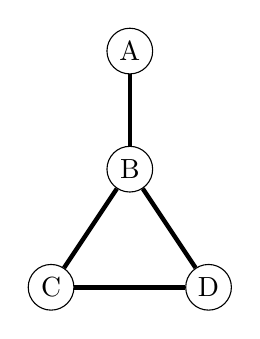
\begin{tikzpicture}
        \node [draw, circle, fill=white, inner sep=4pt, font=\bfseries] (Na) at (1,  0) {\vphantom{1}};
        \node at (Na) {A};
        \node [draw, circle, fill=white, inner sep=4pt, font=\bfseries] (Nb) at (1, -1.5) {\vphantom{1}};
        \node at (Nb) {B};
        \node [draw, circle, fill=white, inner sep=4pt, font=\bfseries] (Nc) at (0, -3) {\vphantom{1}};
        \node at (Nc) {C};
        \node [draw, circle, fill=white, inner sep=4pt, font=\bfseries] (Nd) at (2, -3) {\vphantom{1}};
        \node at (Nd) {D};

        \draw [ultra thick] (Na) -- (Nb);
        \draw [ultra thick] (Nb) -- (Nc);
        \draw [ultra thick] (Nc) -- (Nd);
        \draw [ultra thick] (Nb) -- (Nd);
    \end{tikzpicture}

    \begin{itemize}
        \item <2-> Only find solutions where $C < D$.
        \item <3-> What about for arbitrary symmetries, in both pattern and target graphs?
        \item <4-> Dynamic symmetries?
    \end{itemize}
\end{frame}

\begin{frame}{Counting and Sampling}
    \begin{itemize}
        \item We can easily enumerate all solutions.
        \item If we only need a count, can we speed things up?
        \item <2-> What if an approximate count is OK?
        \item <3-> What if we want a few solutions, but sampled uniformly?
            \begin{itemize}
                \item Common in term-rewriting systems.
            \end{itemize}
        \item <4-> How does this interact with symmetries and decomposition?
    \end{itemize}
\end{frame}

\begin{frame}{Proof Logging}
    \begin{tikzpicture}
        \node (solver) [ inner xsep=4em, inner ysep=2.5em, draw, rounded corners=3pt] { Solver };
        \node (elaborator) [ right=2cm of solver.north east, anchor=north west, inner
        xsep=0.25em, draw, rounded corners=3pt, minimum height=12em, text width=5em, text centered,
        visible on=<3->] {
            \only<1-4>{Checker}\only<5->{Elaborator} };
        \node (verifiedchecker) [ right=2cm of elaborator.north east, anchor=north west, inner
            xsep=0.25em, draw, rounded corners=3pt, minimum height=8em, text width=4em, text
            centered, yshift=-2cm, visible on=<6->] { Verified Checker };

        \node (print) [anchor=south, above=0cm of solver.south, visible on=<2->] { added print statements };
        \draw [dotted, visible on=<2->] (solver.west|-print.north) -- (solver.east|-print.north);

        \draw [->, thick] (solver.east) -- (solver.east -| elaborator.west) coordinate [midway] (solutionmid) node [above, midway] { Result };

        \draw [->, thick, rounded corners=3pt, visible on=<2->] (solver.south) -- (solver.south |- elaborator.west) -- (elaborator.west) coordinate [midway] (proofmid);

        \coordinate (prooflabel) at (proofmid-|solutionmid); \node [above=0cm of prooflabel, visible
        on=<2->] { Proof };

        \coordinate [right=2cm of verifiedchecker.east] (verified);
        \draw [->, thick, visible on=<6->] (verifiedchecker.east) -- (verified)
            node [above, midway] { \textcolor{uofglawn}{\ding{51}} or \textcolor{uofgpillarbox}{\ding{55}} }
            node [below, midway, text centered, text width=5em] { Trusted Result };

        \coordinate [left=1.5cm of solver.west] (input);
        \draw [->, thick] (input) -- (solver.west) coordinate [midway] (inputmid) node [above, midway] { Input };

        \coordinate (verifiedcheckertopleft) at ($(verifiedchecker.west)+($(0cm,1.2cm)$)$);
        \draw [->, thick, visible on=<5->] (elaborator.east |- verifiedcheckertopleft) -- (verifiedcheckertopleft) node [above, midway, text width=4em, text centered] { Result };
        \draw [->, thick, visible on=<5->] (elaborator.east |- verifiedchecker.west) -- (verifiedchecker.west) node [above, midway, text width=4em, text centered] { Kernel Proof };

        \coordinate (elaboratorbotleft) at ($(elaborator.west)+($(elaborator.west)-(solver.east-|elaborator.west)$)$);
        \coordinate (verifiedcheckerbotleft) at ($(verifiedchecker.west)+($(0cm,-1.2cm)$)$);

        \draw [->, thick, rounded corners=3pt, visible on=<3->] ($(inputmid)+(-0.2,0)$) -- (inputmid) -- (inputmid |- elaboratorbotleft) -- (elaboratorbotleft);
        \draw [->, thick, rounded corners=3pt, visible on=<6->] ($(inputmid)+(-0.2,0)$) -- (inputmid) -- (inputmid |- verifiedcheckerbotleft) -- (verifiedcheckerbotleft);

        \coordinate (elaboratortopright) at ($(elaborator.east)+($(verifiedcheckertopleft)-(verifiedchecker.west)$)$);
        \draw [->, thick, visible on=<4->] (elaboratortopright) -- (elaboratortopright-|verifiedchecker.west)
            node [above, midway] { \textcolor{uofglawn}{\ding{51}} or \textcolor{uofgpillarbox}{\ding{55}} };
    \end{tikzpicture}
\end{frame}

\begin{frame}{Components}
    \begin{itemize}
        \item What if the target graph has two components?
        \item <2-> What if the pattern graph has two components?
        \item <3-> What if the graphs are ``nearly'' two components?
    \end{itemize}
\end{frame}

\begin{frame}{Learning}
    \begin{itemize}
        \item Backtracking is bad. We should do CDCL!
        \item Except it doesn't seem to work very well\ldots
    \end{itemize}
\end{frame}

\begin{frame}{Inference on Fancy Graphs}
    \begin{itemize}
        \item What's the equivalent of neighbourhood degree sequence for directed graphs?
        \item What about if we have labels?
        \item Can these be computed efficiently?
    \end{itemize}
\end{frame}

\begin{frame}{Automatic Configuration}
    \begin{itemize}
        \item What if the pattern graph is a triangle? A claw? One edge and one non-edge? A large
            clique?
        \item <2-> Which supplemental graphs should we use?
        \item <2-> Which inference rules are helpful?
    \end{itemize}
\end{frame}

\begin{frame}{Presolving}
    \begin{itemize}
        \item Constraint programming solvers take too long to start up for ``really easy'' instances.
        \item Run a ``fast'' solver for 0.1s and then switch?
        \item <2-> Doesn't help us for very solution-dense enumeration problems though.
    \end{itemize}
\end{frame}

\begin{frame}{Performance Portability}
    \begin{itemize}
        \item Will algorithms designed on this year's hardware work well next year?
        \item <2-> Or on Mac ARM hardware rather than Intel / AMD x64?
        \item <3-> On heterogeneous multi-core?
    \end{itemize}
\end{frame}

\begin{frame}{File Formats}
    \begin{itemize}
        \item Design a graph file format that isn't terrible.
    \end{itemize}
\end{frame}

{
    \usebackgroundtemplate{
        \tikz[overlay, remember picture]
        \node[at=(current page.south), anchor=south, yshift=-1cm, inner sep=0pt]{\includegraphics[keepaspectratio=true, width=\paperwidth]{../../images/background2.jpg}};
    }

    \begin{frame}[plain,noframenumbering]
        \begin{tikzpicture}[remember picture, overlay]
            \node at (current page.north west) {
                \begin{tikzpicture}[remember picture, overlay]
                    \fill [fill=uofguniversityblue, anchor=north west] (0, 0) rectangle (\paperwidth, -2.8cm);
                \end{tikzpicture}
            };

            \node (logo) [anchor=north east, shift={(-0.8cm,-0.2cm)}] at (current page.north east) {
                \includegraphics[keepaspectratio=true,scale=0.5]{../../images/UoG_keyline.pdf}
            };

            \node (logo2) [anchor=north, below=0.2cm of logo.south] {
                \includegraphics[keepaspectratio=true,scale=0.1]{../../images/RAEngWhite.pdf}
            };

            \coordinate (logos) at ($(logo.south)!0.5!(logo2.north)$);

            \node [anchor=west, xshift=0.8cm] at (current page.west |- logos) {
                \begin{minipage}{0.60\paperwidth}\raggedright
                    \textcolor{white}{\url{https://ciaranm.github.io/}} \\[0.3cm]
                    \textcolor{white}{\href{mailto:ciaran.mccreesh@glasgow.ac.uk}{\nolinkurl{ciaran.mccreesh@glasgow.ac.uk}}}
                \end{minipage}
            };
        \end{tikzpicture}
    \end{frame}
}

\end{document}

